%%%%%%%%%%%%%%%%%%%%%%%%%%%%%%%%%%%%%%%%%
% Masters Thesis 
% LaTeX Template
%
% This template is based on a template by:
% Steve Gunn (http://users.ecs.soton.ac.uk/srg/softwaretools/document/templates/)
% Sunil Patel (http://www.sunilpatel.co.uk/thesis-template/)
%
% Template license:
% CC BY-NC-SA 3.0 (http://creativecommons.org/licenses/by-nc-sa/3.0/)
%
%%%%%%%%%%%%%%%%%%%%%%%%%%%%%%%%%%%%%%%%%

%----------------------------------------------------------------------------------------
%	PACKAGES AND OTHER DOCUMENT CONFIGURATIONS
%----------------------------------------------------------------------------------------

\documentclass[
11pt, % The default document font size, options: 10pt, 11pt, 12pt
%oneside, % Two side (alternating margins) for binding by default, uncomment to switch to one side
english, % ngerman for German
singlespacing, % Single line spacing, alternatives: onehalfspacing or doublespacing
%draft, % Uncomment to enable draft mode (no pictures, no links, overfull hboxes indicated)
%nolistspacing, % If the document is onehalfspacing or doublespacing, uncomment this to set spacing in lists to single
liststotoc, % Uncomment to add the list of figures/tables/etc to the table of contents
%toctotoc, % Uncomment to add the main table of contents to the table of contents
%parskip, % Uncomment to add space between paragraphs
%nohyperref, % Uncomment to not load the hyperref package
headsepline, % Uncomment to get a line under the header
%chapterinoneline, % Uncomment to place the chapter title next to the number on one line
%consistentlayout, % Uncomment to change the layout of the declaration, abstract and acknowledgements pages to match the default layout
]{MastersDoctoralThesis} % The class file specifying the document structure

\usepackage[utf8]{inputenc} % Required for inputting international characters
\usepackage[T1]{fontenc} % Output font encoding for international characters

\usepackage{mathpazo} % Use the Palatino font by default
\usepackage{xcolor}

\usepackage{hyperref}
\usepackage{dirtree}
\usepackage[font=small]{caption}
\captionsetup{justification=raggedright,singlelinecheck=false}

\usepackage[backend=bibtex,style=numeric,natbib=true]{biblatex} % Use the bibtex backend with the authoryear citation style (which resembles APA)

\addbibresource{bibliography.bib} % The filename of the bibliography

\usepackage[autostyle=true]{csquotes} % Required to generate language-dependent quotes in the bibliography

%----------------------------------------------------------------------------------------
%	MARGIN SETTINGS
%----------------------------------------------------------------------------------------

\geometry{
	paper=a4paper, % Change to letterpaper for US letter
	inner=2.5cm, % Inner margin
	outer=3.8cm, % Outer margin
	bindingoffset=.5cm, % Binding offset
	top=1.5cm, % Top margin
	bottom=1.5cm, % Bottom margin
	%showframe, % Uncomment to show how the type block is set on the page
}

%----------------------------------------------------------------------------------------
%	THESIS INFORMATION
%----------------------------------------------------------------------------------------

\thesistitle{Man-made Structures Detection from Space} % Your thesis title, this is used in the title and abstract, print it elsewhere with \ttitle
\supervisor{Dr. Jordi \textsc{Vitria}} % Your supervisor's name, this is used in the title page, print it elsewhere with \supname
\examiner{} % Your examiner's name, this is not currently used anywhere in the template, print it elsewhere with \examname
\degree{} % Your degree name, this is used in the title page and abstract, print it elsewhere with \degreename
\author{Peter \textsc{Weber}} % Your name, this is used in the title page and abstract, print it elsewhere with \authorname
\addresses{} % Your address, this is not currently used anywhere in the template, print it elsewhere with \addressname

\subject{Data Science} % Your subject area, this is not currently used anywhere in the template, print it elsewhere with \subjectname
\keywords{} % Keywords for your thesis, this is not currently used anywhere in the template, print it elsewhere with \keywordnames
\university{\href{http://www.ub.edu}{Universitat de Barcelona}} % Your university's name and URL, this is used in the title page and abstract, print it elsewhere with \univname
\department{\href{http://department.university.com}{}} % Your department's name and URL, this is used in the title page and abstract, print it elsewhere with \deptname
\group{\href{http://researchgroup.university.com}{}} % Your research group's name and URL, this is used in the title page, print it elsewhere with \groupname
\faculty{\href{http://mat.ub.edu}{Facultat de Matemàtiques i Informàtica}} % Your faculty's name and URL, this is used in the title page and abstract, print it elsewhere with \facname

\AtBeginDocument{
\hypersetup{pdftitle=\ttitle} % Set the PDF's title to your title
\hypersetup{pdfauthor=\authorname} % Set the PDF's author to your name
\hypersetup{pdfkeywords=\keywordnames} % Set the PDF's keywords to your keywords
}

\begin{document}

\frontmatter % Use roman page numbering style (i, ii, iii, iv...) for the pre-content pages

\pagestyle{plain} % Default to the plain heading style until the thesis style is called for the body content

%----------------------------------------------------------------------------------------
%	TITLE PAGE
%----------------------------------------------------------------------------------------

\begin{titlepage}
\begin{center}

\vspace*{.06\textheight}
{\scshape\LARGE \univname\par}\vspace{1.5cm} % University name
\textsc{\Large Fundamentals of Data Science Master's Thesis}\\[0.5cm] % Thesis type

\HRule \\[0.4cm] % Horizontal line
{\huge \bfseries \ttitle\par}\vspace{0.4cm} % Thesis title
\HRule \\[1.5cm] % Horizontal line
 
\begin{minipage}[t]{0.4\textwidth}
\begin{flushleft} \large
\emph{Author:}\\
\href{http://www.johnsmith.com}{\authorname} % Author name - remove the \href bracket to remove the link
\end{flushleft}
\end{minipage}
\begin{minipage}[t]{0.4\textwidth}
\begin{flushright} \large
\emph{Supervisor:} \\
\href{http://www.jamessmith.com}{\supname} % Supervisor name - remove the \href bracket to remove the link  
\end{flushright}
\end{minipage}\\[3cm]
 
\vfill

\large \textit{A thesis submitted in partial fulfillment of the requirements\\ for the degree of MSc in Fundamentals of Data Science}\\[0.3cm] % University requirement text
\textit{in the}\\[0.4cm]
\facname\\[2cm] % Research group name and department name
 
\vfill

{\large \today}\\[4cm] % Date
%\graphics{Logo} % University/department logo - uncomment to place it
 
\vfill
\end{center}
\end{titlepage}


%----------------------------------------------------------------------------------------
%	ABSTRACT PAGE
%----------------------------------------------------------------------------------------

\begin{abstract}
\addchaptertocentry{\abstractname} % Add the abstract to the table of contents
The Thesis Abstract is written here (and usually kept to just this page). The page is kept centered vertically so can expand into the blank space above the title too\ldots
\end{abstract}

%----------------------------------------------------------------------------------------
%	ACKNOWLEDGEMENTS
%----------------------------------------------------------------------------------------

\begin{acknowledgements}
\addchaptertocentry{\acknowledgementname} % Add the acknowledgements to the table of contents
The acknowledgments and the people to thank go here, don't forget to include your project advisor\ldots
\end{acknowledgements}



%----------------------------------------------------------------------------------------
%	THESIS CONTENT - CHAPTERS
%----------------------------------------------------------------------------------------

\mainmatter % Begin numeric (1,2,3...) page numbering

\pagestyle{thesis} % Return the page headers back to the "thesis" style

% Include the chapters of the thesis as separate files from the Chapters folder
% Uncomment the lines as you write the chapters

Report structure:

\begin{enumerate}

	\item Chapter 1: Introduction
		\begin{itemize}
			\item Problem introduction, satellites, Satellogic, motivation
			\item Previous work, literature
		\end{itemize}
		
	\item Chapter 2: Building datasets
		\begin{itemize}
			\item Existing datasets
			\item Google Maps
			\item USGS, land cover
		\end{itemize}
		
	\item Chapter 3: Gist approach
		\begin{itemize}
			\item Features
			\item Model
			\item Results
		\end{itemize}
		
	\item Chapter 4: DL approach
		\begin{itemize}
			\item Features
			\item Model
			\item Results
		\end{itemize}
	
	\item Chapter 5: Final results
		\begin{itemize}
			\item Results
			\item Cost
			\item Environment impact
		\end{itemize}
		
	\item Chapter 6: Conclusion
	
\end{enumerate}

\tableofcontents

%% Chapter 1

\chapter{Introduction} % Main chapter title

\label{Chapter1} % For referencing the chapter elsewhere, use \ref{Chapter1} 

%----------------------------------------------------------------------------------------

% Define some commands to keep the formatting separated from the content 
\newcommand{\keyword}[1]{\textbf{#1}}
\newcommand{\tabhead}[1]{\textbf{#1}}
\newcommand{\code}[1]{\texttt{#1}}
\newcommand{\file}[1]{\texttt{\bfseries#1}}
\newcommand{\option}[1]{\texttt{\itshape#1}}

%----------------------------------------------------------------------------------------

\section{Motivation}

BigEarthNet Motivation:
Existing Remote Sensing Datasets contain a small number of annotated images and therefore do not suffice to train a complex ConvNet with many different parameters.
Remote sensing versus Computer (Using pretrained nets on ImageNet)


BagOfVisualWords: useless



Extreme value theory-based calibration: useless




Climate Change, population control, ilegal habitat/ilegal land use


\section{Satellogic}




\section{Thesis Outline}
% Chapter 1

\chapter{Building Datasets} % Main chapter title

\label{Chapter2} % For referencing the chapter elsewhere, use \ref{Chapter1} 

%----------------------------------------------------------------------------------------

% Define some commands to keep the formatting separated from the content 
\newcommand{\keyword}[1]{\textbf{#1}}
\newcommand{\tabhead}[1]{\textbf{#1}}
\newcommand{\code}[1]{\texttt{#1}}
\newcommand{\file}[1]{\texttt{\bfseries#1}}
\newcommand{\option}[1]{\texttt{\itshape#1}}

In this chapter, we will give an overview of existing (labelled) aerial imagery datasets and outline the reasons why none of them is suitable for our investigation. Following this discussion, we will describe two approaches for obtaining our own labelled dataset.

\section{Requirements and Considerations}

Before we go into the presentation of existing labelled datasets we discuss the requirements that the dataset needs to fulfill in order to serve for the investigation in this thesis project. As a refresher, we want to detect human impact on aerial images and determine the dependency on resolution per pixel of a chosen evaluation metric. Ideally, the range for the resolutions should scale from a few tens of centimeters to a few tens of meters, whereas the images with low resolution can be generated from the high resolution images by downsampling. Having in mind previous arguments, we mainly need to consider three aspects. 

First, we need to have imagery data with labels that can be used to clearly distinguish between existing and non-existing human impact, respectively. This impact might be classified pixel wise, or as binary classification for the entire image, or as multi-class classification that can be translated into binary labelling. Second, 
we need a balanced dataset of approximately the same number of images for both labels, and variations of the images as large as possible with respect to different terrains. Third, the images need to have a resolution per pixel which is equal or better than 1m. Also, the height and width of the images should measure at least $500\times500$ pixels, so that one has enough room for downsampling. 

\section{Existing Datasets}

In table \ref{table:datasets} we have summarized the most relevant remote sensing datasets with ground truth labels, that can be found in literature. The table  lists the name of the dataset together with the bibliographic reference. It also details the data source for the images. Further it contains a description about the number of images, the resolution of the images, the size (in pixel) of the images where images are squared, and the number of categories.

The datasets were collected using different publicly available data sources. These range from pure low resolution satellite imagery (Sentinel-2) to high-resolution images taken with an aircraft (USGS) to a mix of different image sources (Google Earth). 

The satellite images have a resolution of equal or larger than 10~m and they are collected with the Sentinel-2 satellites of the European Earth observation program Copernicus. Although the datasets from this source (BigEarthNet and EuroSat) are comparatively large, they do not suffice for our purpose, because the resolution is not good enough and the images are too small.

\begin{table}[h!]
	\begin{tabular}{l | l | l | l | l | l }
	name & source & images & resolution (m) & size (pixel) & categories \\
	\hline
	BigEarthNet \parencite{sumbul2019} & Sentinel-2 & 590,326 & 10, 20, 60 & 120, 60, 20 & $\sim$ 50 \\
	EuroSAT \parencite{helber2017}	& Sentinel-2 & 27,000  & 10 & 64  & 10 \\
	UCMerced \parencite{yang2010} & USGS & 2100 & 0.3 & 256 & 21 \\
	DeepSat \parencite{basu2015}  & USGS  & 405,000 & 1 & 28 & 6  \\
	AID \parencite{xia2016} & Google Earth & 10,000  & 0.5 - 8  & 600 & 30 \\
	PatternNet \parencite{zhou2017} & Google Earth & 30,400 & 0.06 - 4.69 & 256 & 38 \\
	\end{tabular}
	\caption{Publicly available remote sensing datasets with labels.}
	\label{table:datasets}	
\end{table}

The USGS National Map Urban Area Imagery collection \href{https://earthexplorer.usgs.gov/}{(\textit{see link})} was utilized to collect remote sensing datasets in the two works UCMerced and DeepSat, where the former is the dataset that comes closest to our requirements. It has 21 categories of which only 2 belong to images without human impact, while the other 19 show human impact. The DeepSat dataset unfortunately consists of image patches which are only $28 \times 28$ large, so that we aren't able to study these images as a function of resolution.

The datasets using Google Earth as data source are collected using either the Google Earth or the Google Maps API. These images vary in resolution as well as in their original data provider since Google accesses several data sources. 
Both datasets, the AID and the PatternNet dataset, have about 30 categories with several images in each category. Here, different categories have different resolutions per pixel, and again most of the categories relate to urban areas so that we do not have sufficient images without human impact. Even the categories that in principle should not show human influence contain images that break this rule.

Overall, the main issue with these datasets stems from the fact that non of them was collected with the purpose to analyze the human footprint and therefore they are very unbalanced, and do not contain sufficient variety of images for the classes without human influence. Therefore, we decided to collect and label images by ourselfes. In our first approach we used the Google Maps API, and in our final approach we used datasets from the USGS Aerial Imagery collection.

\section{Google Maps}

Google has a public API that allows for querying images from their service Google Maps. In its most basic form, the API accepts as input parameters a lattitude and longitude, a zoom, and the number of pixels to return. Given this set of parameters one can calculate the resolution per pixel (see~\parencite{gmaps_res_per_m}), which is given by
\begin{equation}
\frac{meter}{pixel} = \frac{156543.03392 \cdot cos(\frac{lattitude \cdot \pi}{180})}{2 ^ {zoom}}.
\end{equation}



\section{USGS, Land Cover}

\subsection{Getting the Data}
To be able to construct a balanced and representative dataset we first decided to focus on images of the United States, which allows for a large variety of different terrains. We then used as data source the Aerial Imagery datasets from USGS Earthexplorer \href{https://earthexplorer.usgs.gov/}{(\textit{see link})} which we combined with information about Land Cover and Land Use available from the USGS Land Cover Viewer \href{https://gis1.usgs.gov/csas/gap/viewer/land_cover/Map.aspx}{(\textit{see link})}.

\begin{figure}[h!]
	\centering
	\captionsetup{width=1\linewidth}
	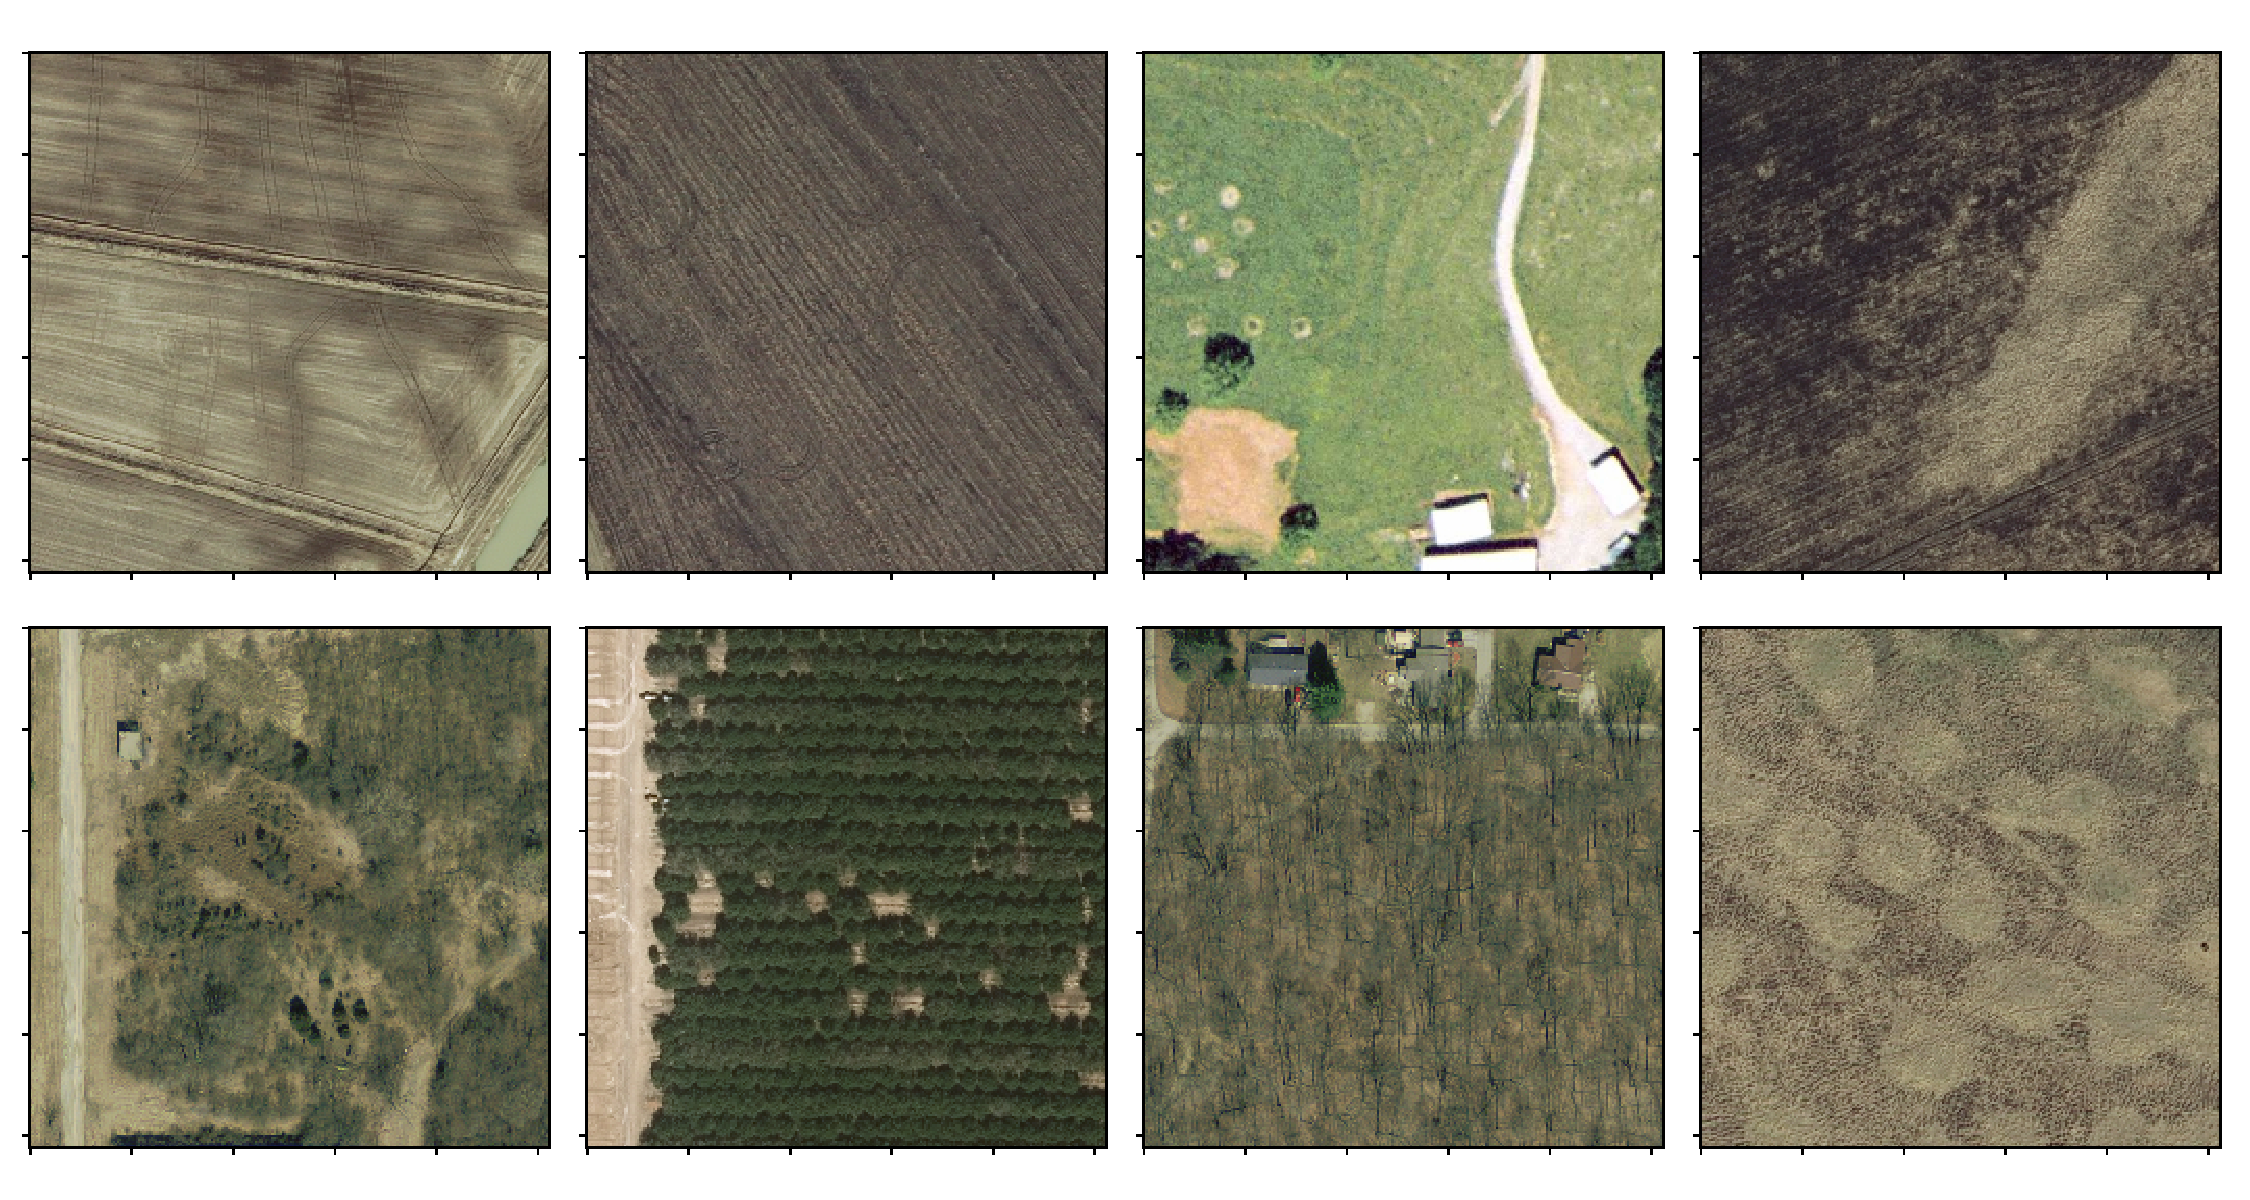
\includegraphics[width=1\textwidth]{Figures/agriculture_sample.pdf}
	\caption{\textbf{Example images of category Agricultue.} All images in this figure show clear signs of human impact. The images have a size of $512\times512$ pixels and a resolution of $0.3$m per pixel.}
	\label{fig:agriculture_sample}
\end{figure}

\begin{figure}[h!]
	\centering
	\captionsetup{width=1\linewidth}
	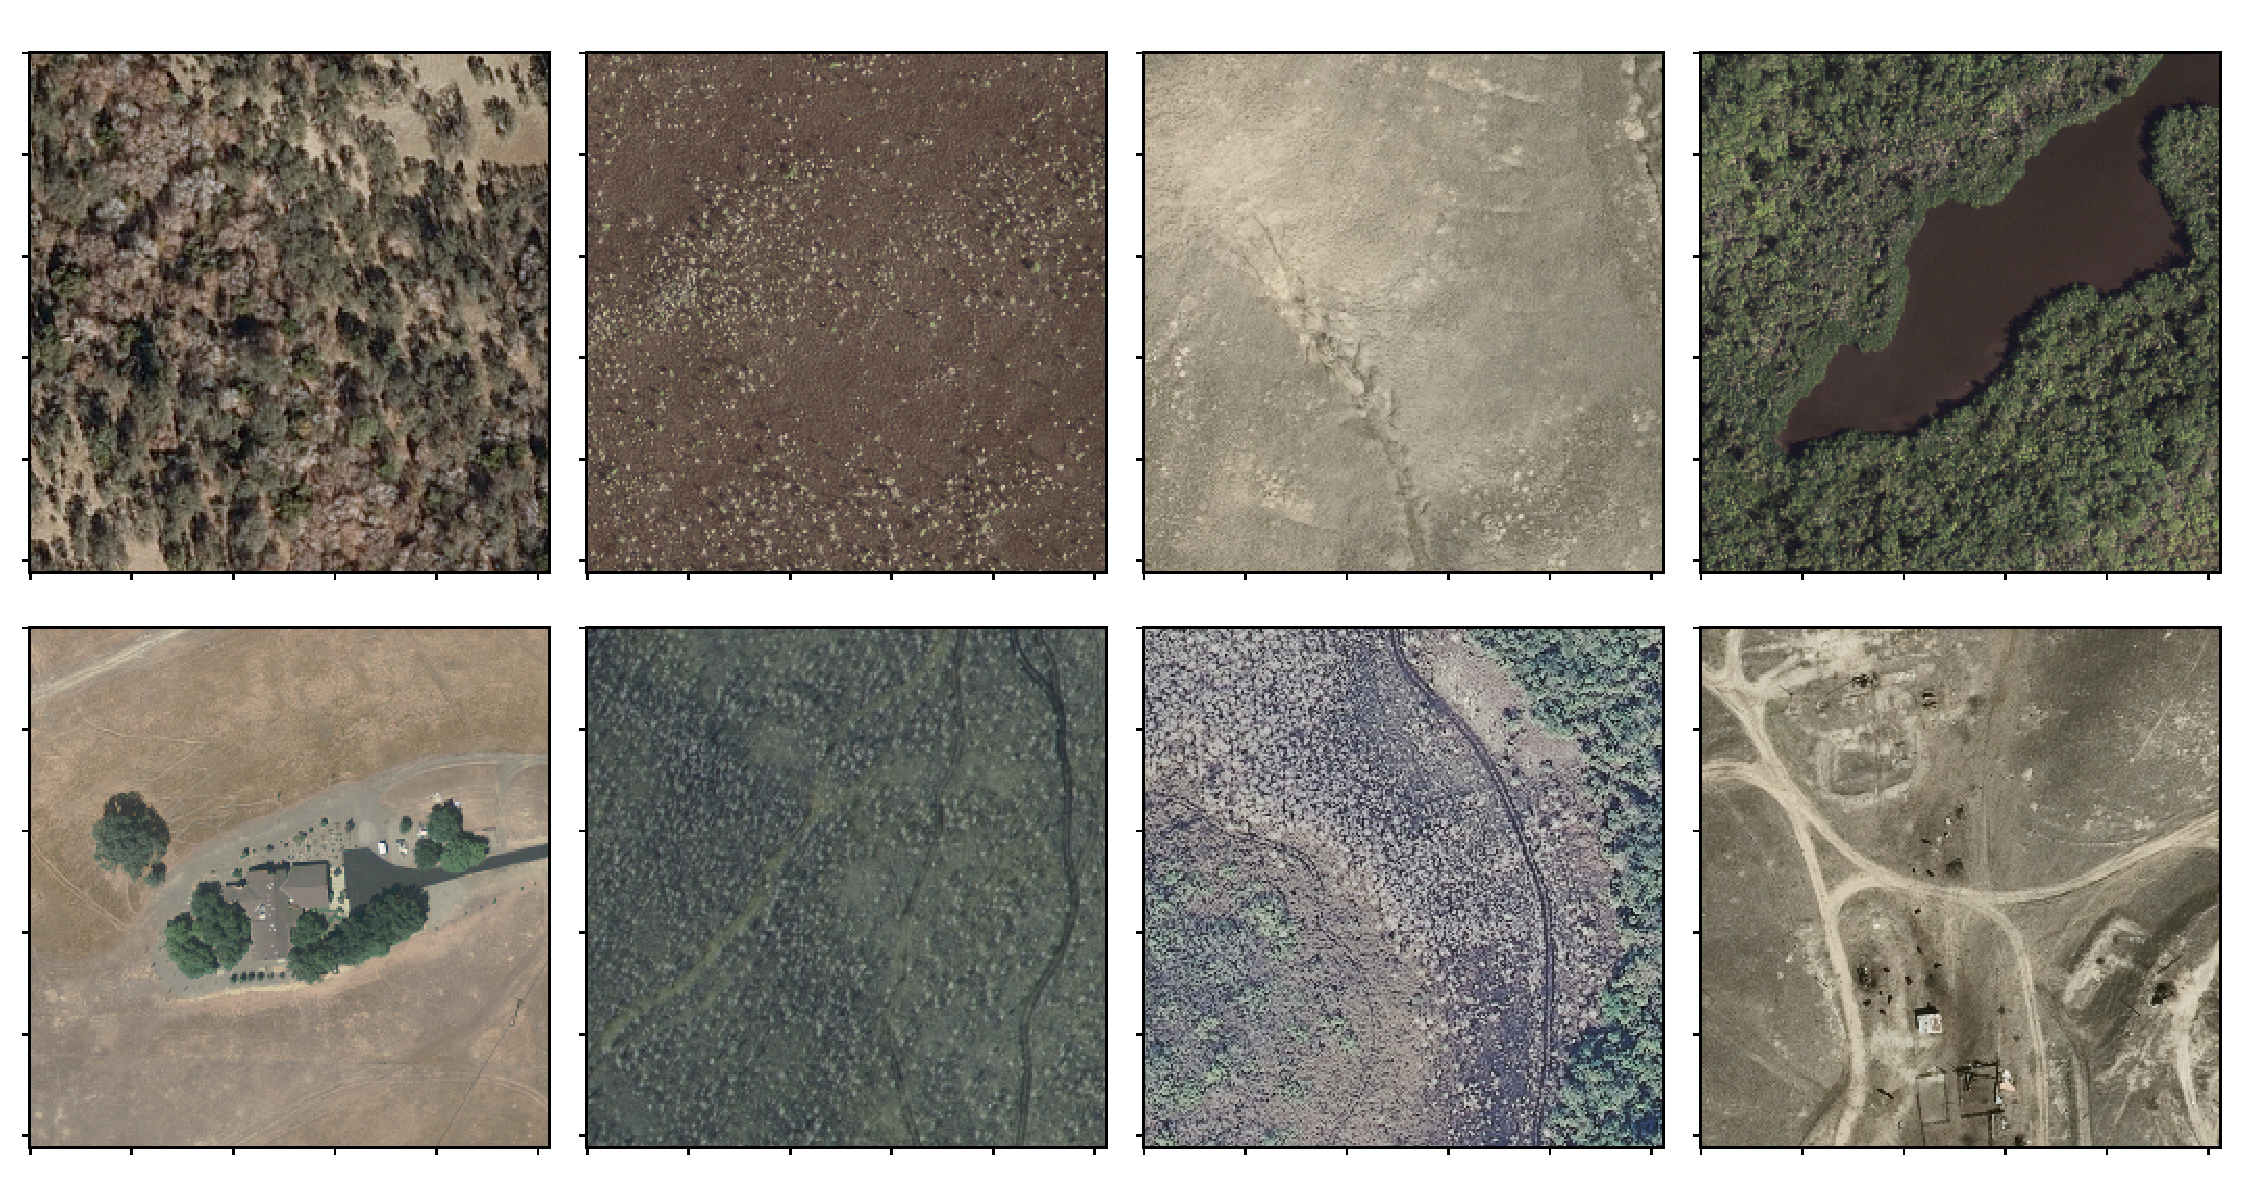
\includegraphics[width=1\textwidth]{Figures/shrubland-grassland_sample.pdf}
	\caption{\textbf{Example images of category Shrubland-grassland.} The images in the first row do not contain any human influence, while the images in the second row show influence by humans. The images in this figure have a size of $512\times512$ pixels and a resolution of $0.3$m per pixel.}
	\label{fig:shrubland-sample}
\end{figure}

\begin{figure}[h!]
	\centering
	\captionsetup{width=1\linewidth}
	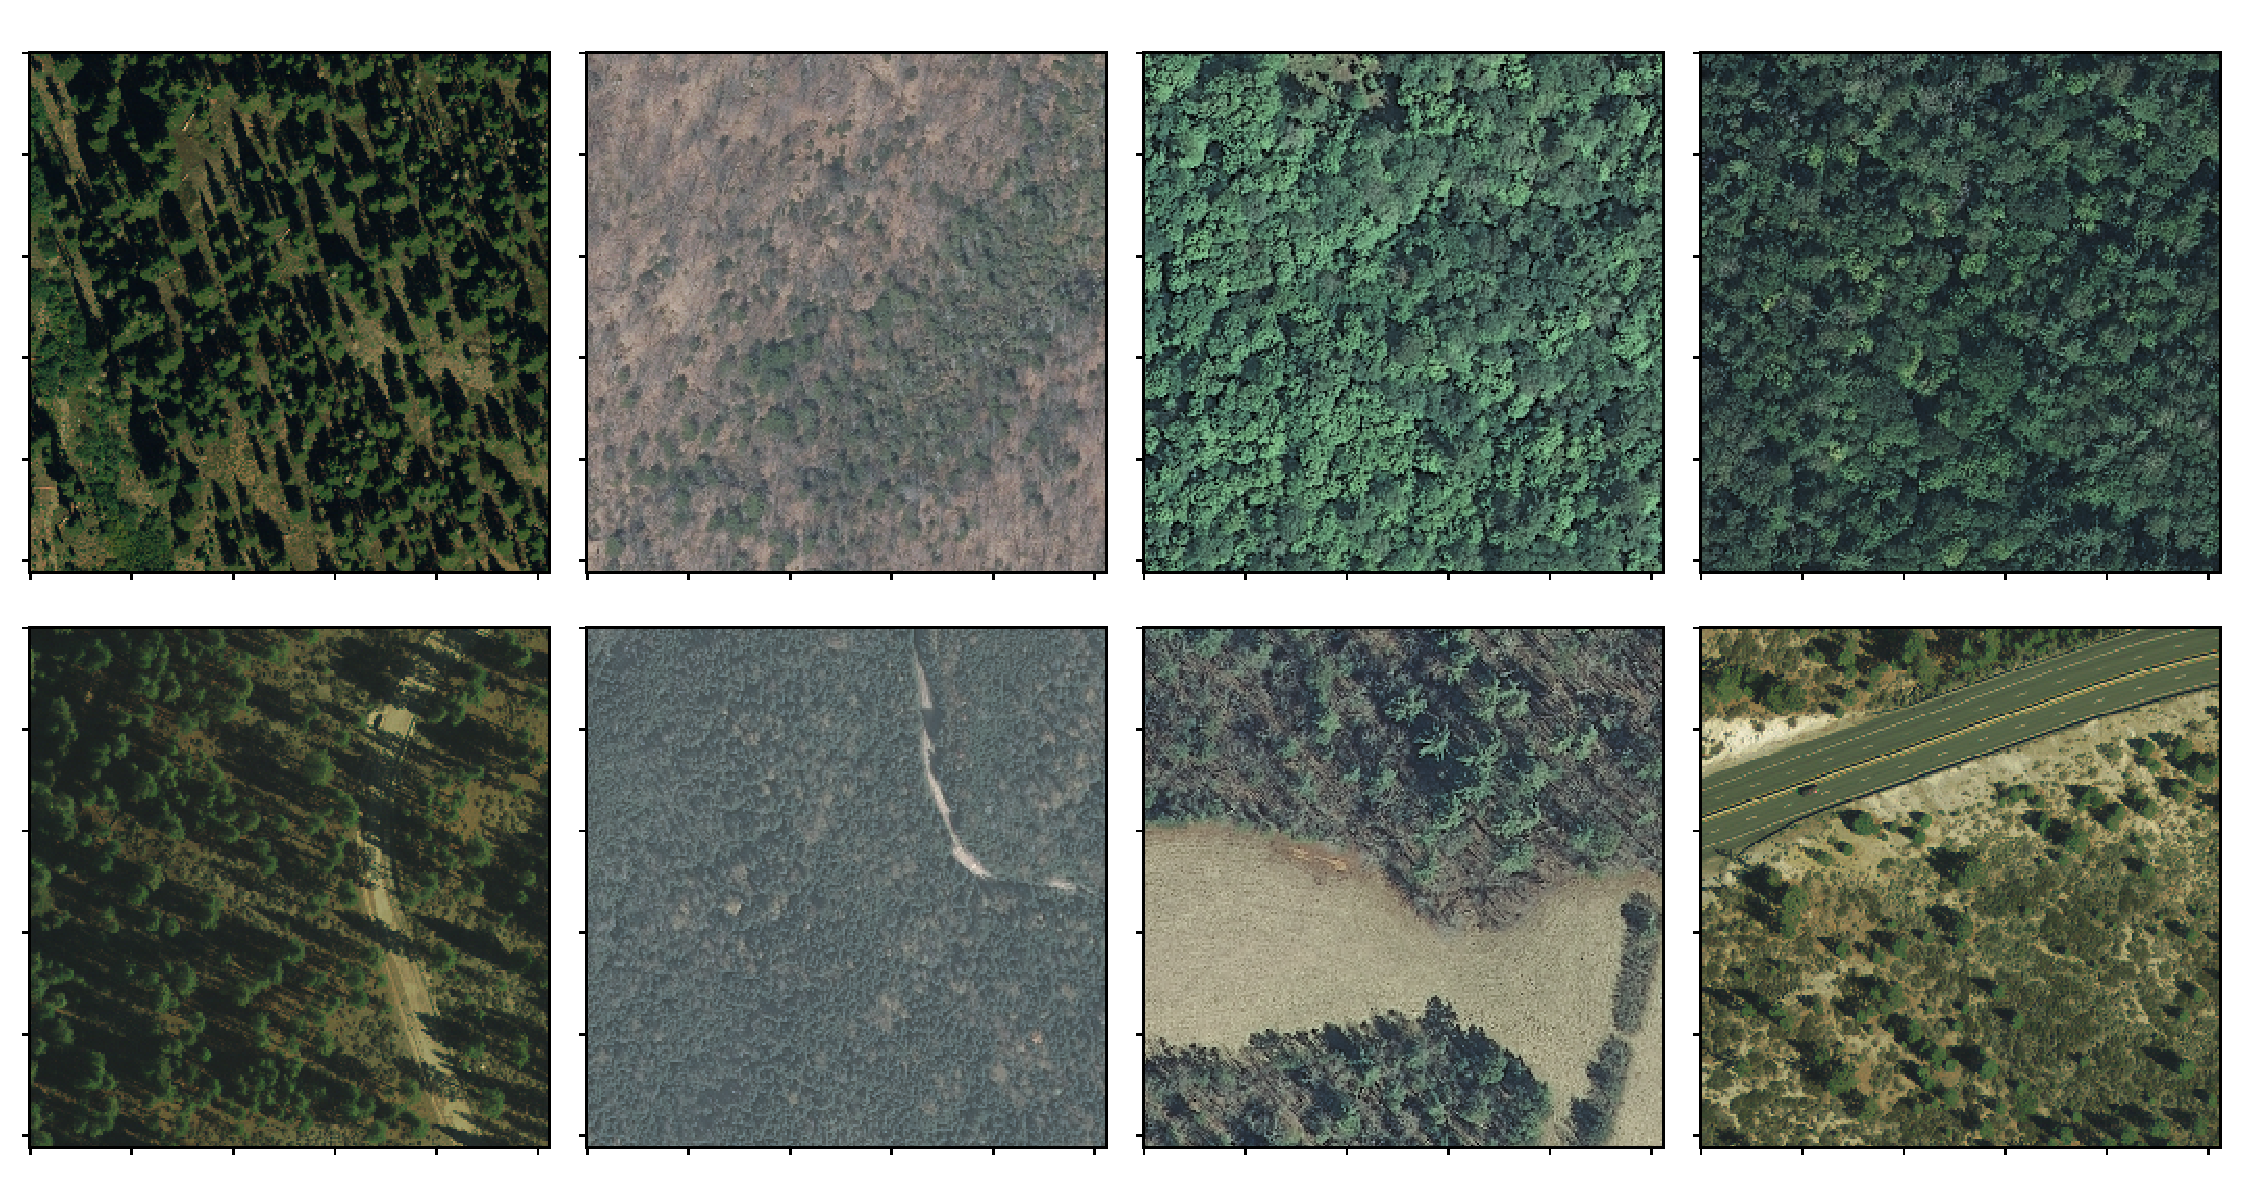
\includegraphics[width=1\textwidth]{Figures/forest-woodland_sample.pdf}
	\caption{\textbf{Example images of category Forest-woodland.} The images in the first row do not contain any human influence, while the images in the second row show influence by humans. The images in this figure have a size of $512\times512$ pixels and a resolution of $0.3$m per pixel.}
	\label{fig:forest-sample}
\end{figure}

\begin{figure}[h!]
	\centering
	\captionsetup{width=1\linewidth}
	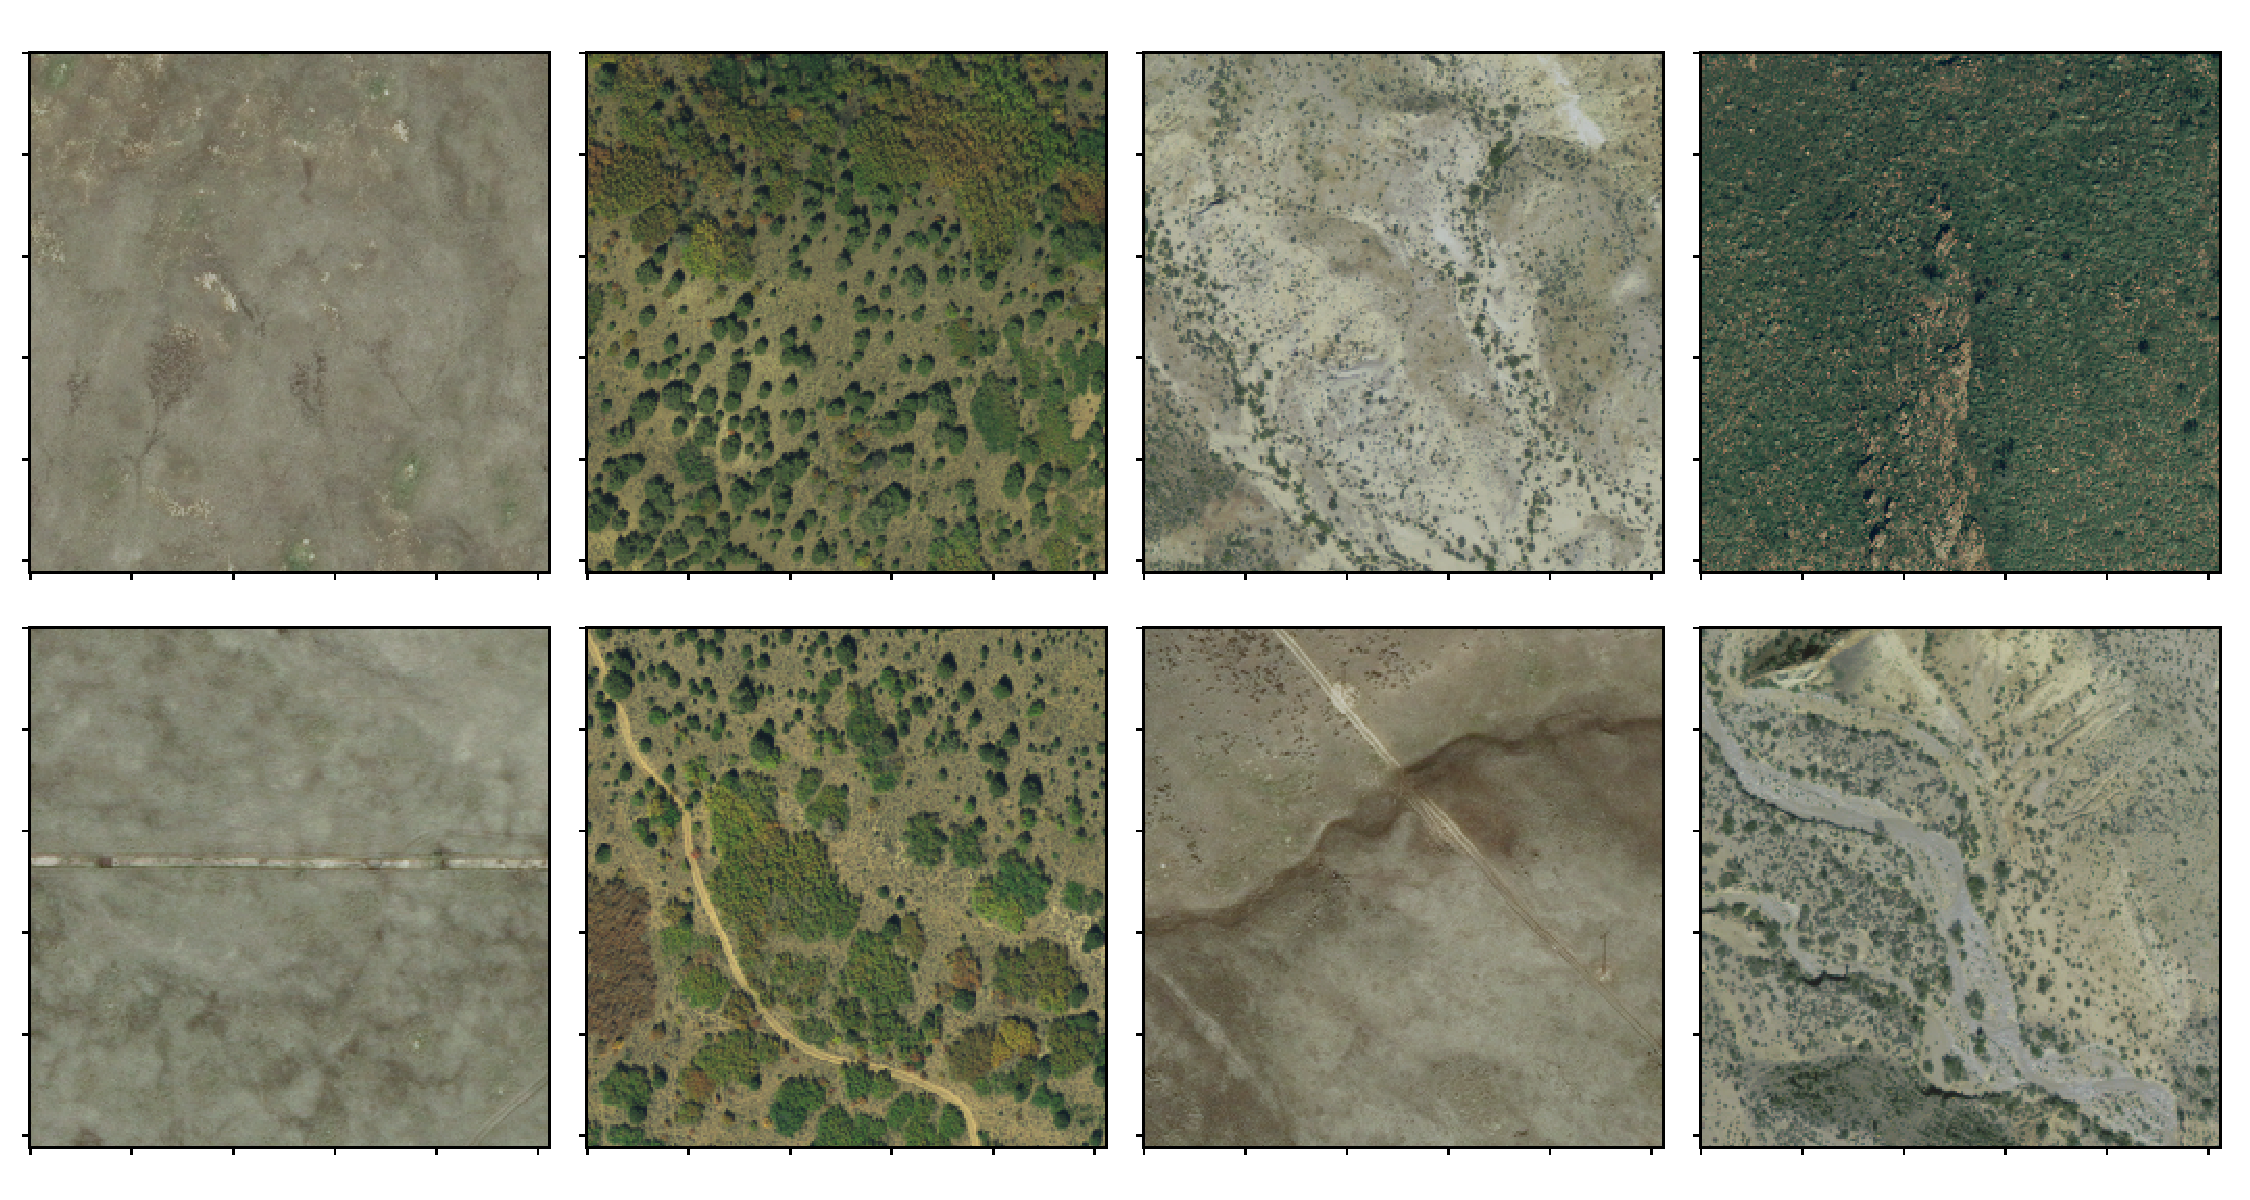
\includegraphics[width=1\textwidth]{Figures/semi-desert_sample.pdf}
	\caption{\textbf{Example images of category Semi-desert.} The images in the first row do not contain any human influence, while the images in the second row show influence by humans. The images in this figure have a size of $512\times512$ pixels and a resolution of $0.3$m per pixel.}
	\label{fig:desert-sample}
\end{figure}

When looking for images we excluded cities and highly developed urban areas, and instead focussed on unpopulated areas. Specifically, we limited our image search to the four Land Use categories Agriculture, Shrubland-Grassland, Semi-Desert, Forest-Woodland that can be found in the USGS Land Cover Viewer. Note that these categories served as a rough geographic reference to pin down geolocations of interest, in order to guarantee a dataset with a good variety of different terrains. We also found that it is harder to find images without human, which is why we selected many images from national parks. However, within a given area/terrain we always tried to have images with and without impact.

Once an area was pointed out as a region of interest, we located it on USGS Earthexplorer and downloaded images from that area. In particular, we constructed two datasets with $0.3m$ and $1m$ resolution, respectively. The former was taken from the category High Resolution Orthoimagery and the latter from the category National Agriculture Imagery Program (NAIP). Note that the images in these categories usually have a height and a width of several thousand pixels, and hence oocupy a few hundreds of Megabytes of disk space. We cropped smaller images out of the raw images, which will be discussed in more detail in the following section. Overall, we downloaded about 100 images for each dataset.


\subsection{Data Processing and Labeling}
Our data processing pipeline consists of the following steps:
\begin{itemize}
	\item Download large raw images
	\item Crop images of size $512\times512$ pixels
	\item Label images with either zero (no human impact), one (minimal human impact), two (obvious human impact)
	\item Degrade images, i.e. reduce number of pixels and thereby resolution per pixel
\end{itemize}

Let us discuss each of these steps in more detail. Every raw image was processed, whereas the processed images of size $512\times512$ were saved in a folder named by its category. Note that every raw image resulted in approximately $100 - 150$ processed images, so that we ended up with more than 10,000 images for each dataset.

Within each category of the processed images we labelled a selected portion of the images, by moving them into the folder with the respective label name. The folder structure we used is the following, where pointy brackets '<parameter>' indicate a parameter and 'etc' stands for the three label folders.

\dirtree{%
	.1 \{raw-images-\}usgs-<pixels>-res<resolution>m.
	.2 semi-desert.
	.3 label-0.
	.3 label-1.
	.3 label-2.
	.2 agriculture.
	.3 label-2.
	.2 shrubland-grassland.
	.3 label-0.
	.3 label-1.
	.3 label-2.
	.2 semi-desert.
	.3 label-0.
	.3 label-1.
	.3 label-2.
}

\begin{figure}[h!]
	\centering
	\captionsetup{width=1\linewidth}
	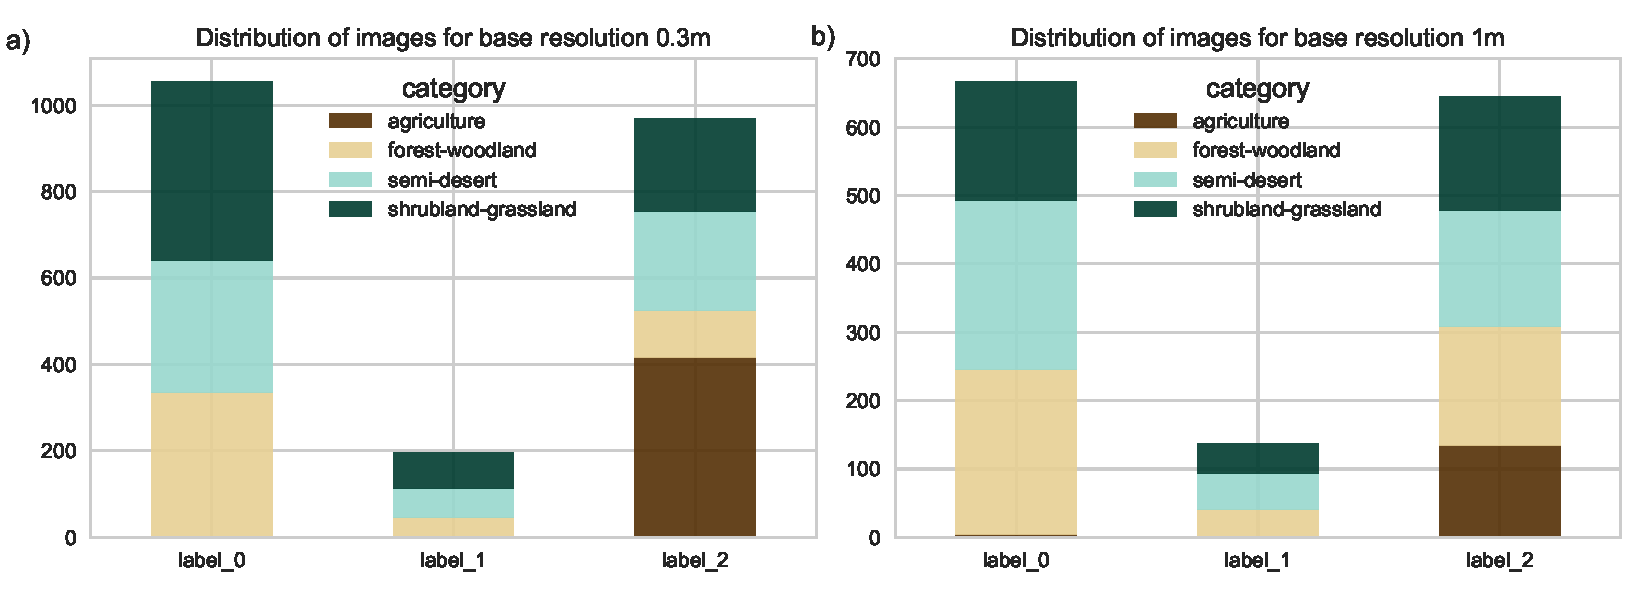
\includegraphics[width=1\textwidth]{Figures/imstats.pdf}
	\caption{\textbf{Number of images per category and label.} (a) Distribution of images for dataset with resolution of 0.3m per pixel. (b) Distribution of images for dataset with resolution of 1m per pixel.}
	\label{fig:imstats}
\end{figure}

When labelling we sticked to the following rules. First, we classified images with no human impact at all into the class with label zero,  while we classified images with very clear human influence into the class with label two. Ambigious images, i.e. images with minimal human trace were classified into label one. Second, we've put major effort into creating datasets that contain images of similar texture spread across all classes. If we for example classified a set of images of a certain forest type into the class with label zero we classified another set of images with a similar forest type, but containing a building or a street, into the class with label two. The same applies for images in class with label one when they contain e.g. a small walking path. We followed the latter rule for all categories except Agriculture. The Agriculture images all show human influence, and were therefore all classified with label two. By sticking to these rules, we are able to guarantee that the algorithm learns features that relate to human impact, and not to image artefacts such as color or texture.

In Figures \ref{fig:agriculture_sample} - \ref{fig:desert-sample} we display sample images for each of the four categories Agriculture, Shrubland-grassland, Forest-woodland and Semi-desert. These images belong to the dataset which has a resolution per pixel of 0.3m. Note that in Figs. \ref{fig:shrubland-sample} - \ref{fig:desert-sample} the first row represents images of label zero and the second row shows images that belong to label two. As mentioned above, the images in Fig.~\ref{fig:agriculture_sample} all contain human influence. 

The distribution of categories and labels is shown in Fig.~\ref{fig:imstats}. Overall, for the 0.3m dataset we classified about 2200 images, and for the 1m dataset we classified about 1450 images. During classification our main goal consisted in creating a balanced dataset between labels zero and two. The minority of images, roughly $10\%$ of all classified images were assigned to label 1. These images were used at random to investigate the behaviour of the Machine Learning classifier, which is discussed in chapter~\ref{Chapter4} \textcolor{red}{VERIFY}.

\begin{figure}[h!]
	\centering
	\captionsetup{width=1\linewidth}
	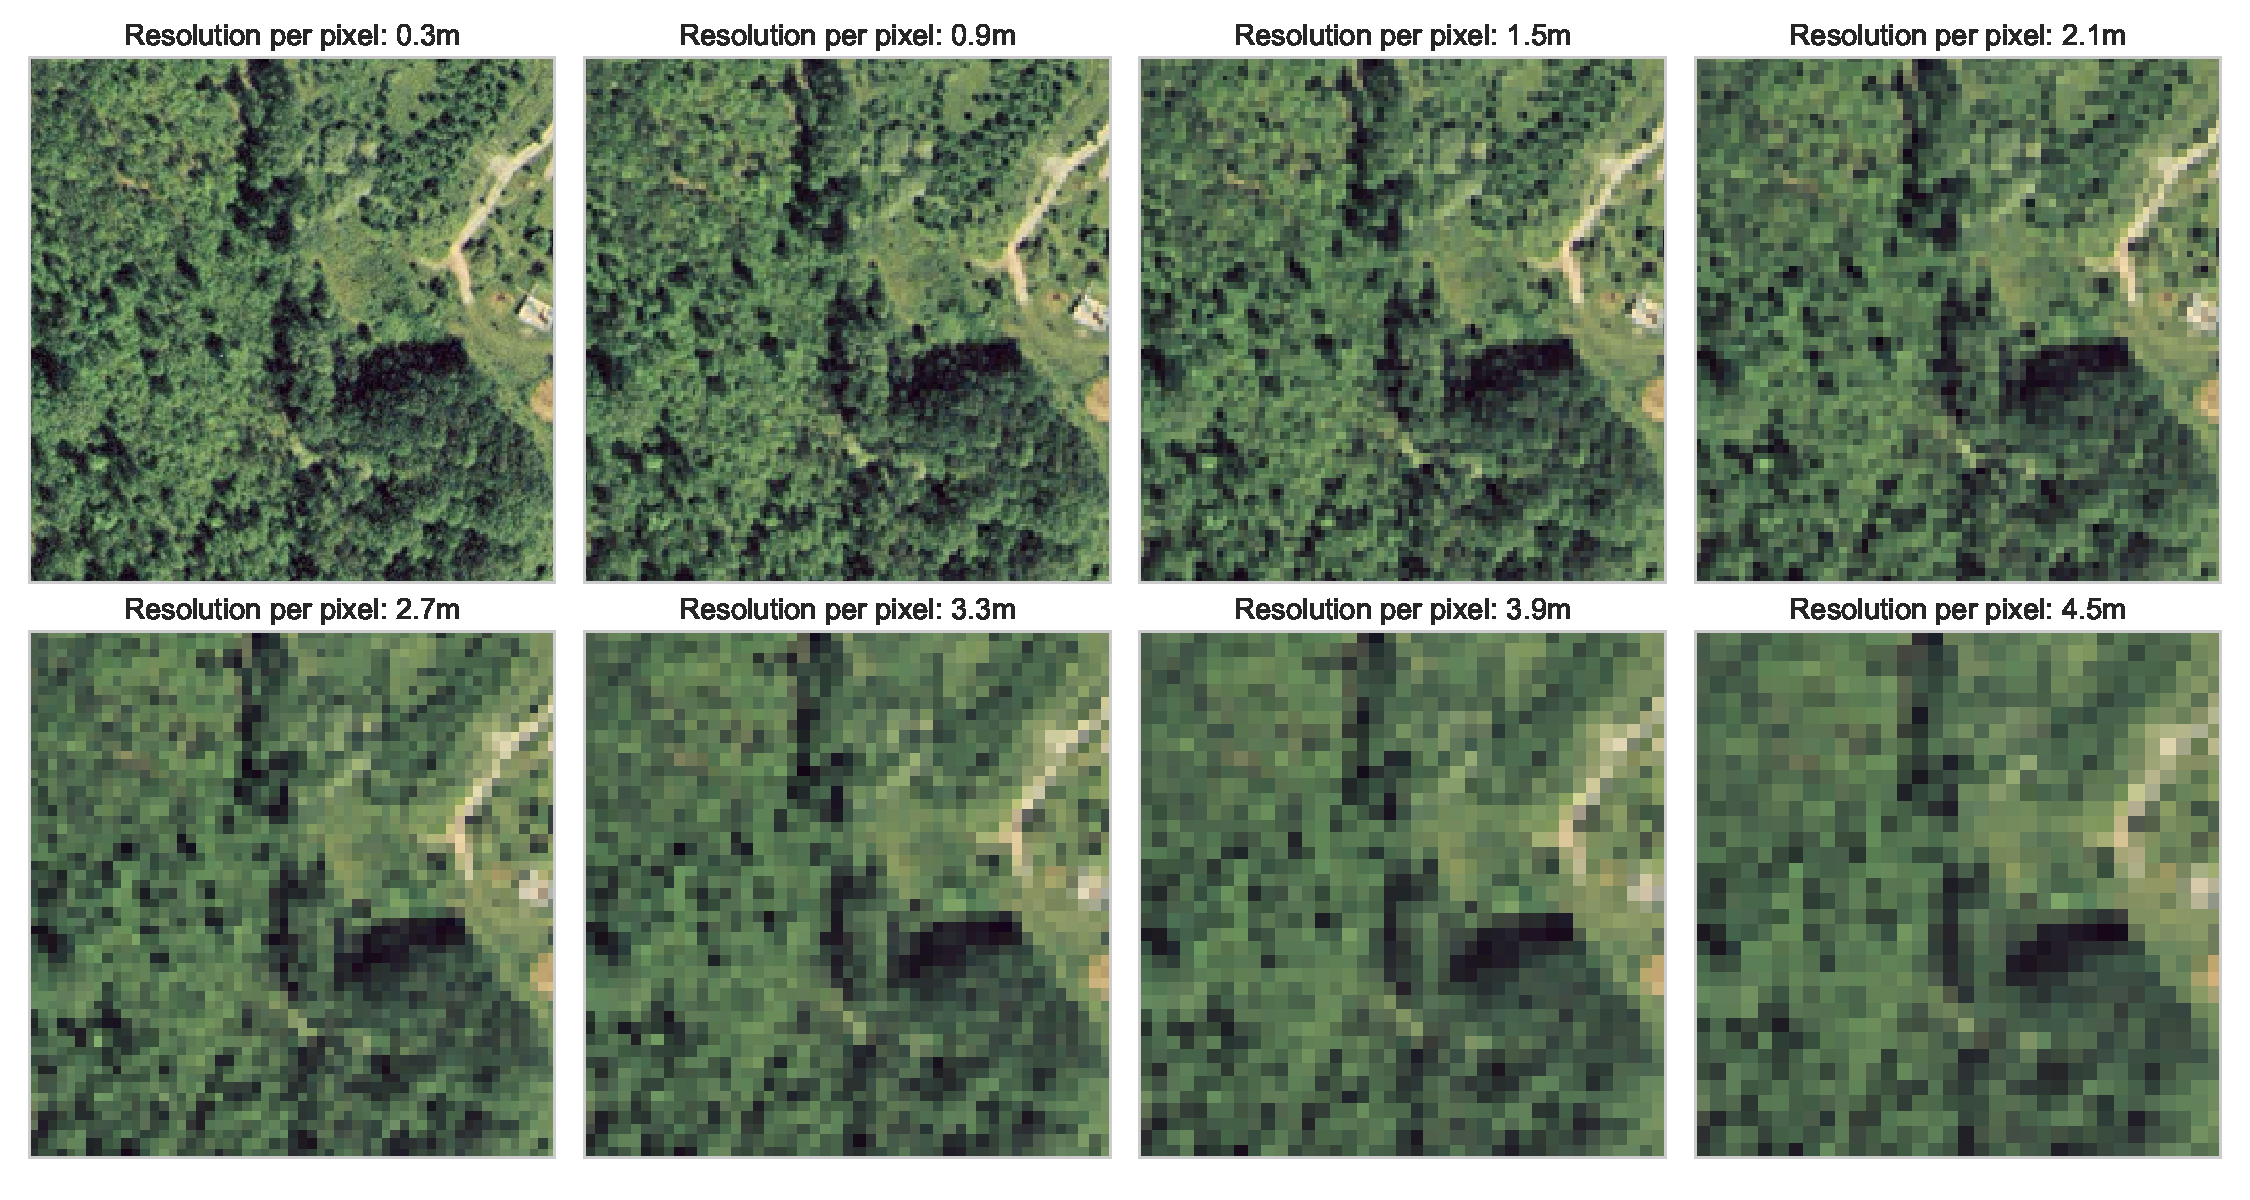
\includegraphics[width=1\textwidth]{Figures/demo_degrade.pdf}
	\caption{\textbf{Example of image downsampling}. The upper left image has the base resolution, 0.3m per pixel, and a size of $512\times512$ pixels whereas the lower right image has the worst resolution, 4.5m per pixel, and a size of $34\times34$ pixels. All intermediate images are downsampled by a factor corresponding to the resolution of the actual image divided by the base resolution. For instance, for the lower right image it is 15.}
	\label{fig:degrade}
\end{figure}

The last step of the data processing pipeline consisted in downsampling the processed and labelled images, to obtain images with a lower resolution per pixel. We used a Lanczos filter \parencite{duchon1979} for the sampling, which is based on a sinusoidal kernel. In Fig.~\ref{fig:degrade}) we show a few selected resolutions for an example image from the agriculture category. Note that here we only schematically depict an example in order to illustrate the process. However, in our Machine Learning pipeline the images are downsampled on the fly and the result of this process is not stored on disk.

For this particular image one can observe how certain image features disappear as the image quality is decreased. Above a resolution of around 3m per pixel one is not able anymore to identify the building close to the right corner of the image. 
The texture of the track that leads up to the building is blurred above a resolution of around 4m per pixel. This shows how different elements in an image are not recognizable anymore once the resolution is worse than their characteristic resolution.



%----------------------------------------------------------------------------------------
 
%% Chapter 1

\chapter{Building Datasets} % Main chapter title

\label{Chapter3} % For referencing the chapter elsewhere, use \ref{Chapter1} 

%----------------------------------------------------------------------------------------

In this chapter, we will give an overview of existing (labelled) aerial imagery datasets and outline the reasons why none of them is suitable for our investigation. Following this discussion, we will describe two approaches for obtaining our own labelled dataset.

\section{Requirements and Considerations}

Before we go into the presentation of existing labelled datasets we discuss the requirements that the dataset needs to fulfill in order to serve for the investigation in this thesis project. As a refresher, we want to detect human impact on aerial images and determine the dependency on resolution per pixel of a chosen evaluation metric. Ideally, the range for the resolutions should scale from a few tens of centimeters to a few tens of meters, whereas the images with low resolution can be generated from the high resolution images by downsampling. Having in mind previous arguments, we mainly need to consider three aspects. 

First, we need to have imagery data with labels that can be used to clearly distinguish between existing and non-existing human impact, respectively. This impact might be classified pixel wise, or as binary classification for the entire image, or as multi-class classification that can be translated into binary labelling. Second, 
we need a balanced dataset of approximately the same number of images for both labels, and variations of the images as large as possible with respect to different terrains. Third, the images need to have a resolution per pixel which is equal or better than 1m. Also, the height and width of the images should measure at least $500\times500$ pixels, so that one has enough room for downsampling. 

\section{Existing Datasets}

In table \ref{table:datasets} we have summarized the most relevant remote sensing datasets with ground truth labels, that can be found in literature. The table  lists the name of the dataset together with the bibliographic reference. It also details the data source for the images. Further it contains a description about the number of images, the resolution of the images, the size (in pixel) of the images where images are squared, and the number of categories.

The datasets were collected using different publicly available data sources. These range from pure low resolution satellite imagery (Sentinel-2) to high-resolution images taken with an aircraft (USGS) to a mix of different image sources (Google Earth). 

The satellite images have a resolution of equal or larger than 10~m and they are collected with the Sentinel-2 satellites of the European Earth observation program Copernicus. Although the datasets from this source (BigEarthNet and EuroSat) are comparatively large, they do not suffice for our purpose, because the resolution is not good enough and the images are too small.

\begin{table}[h!]
	\begin{tabular}{l | l | l | l | l | l }
	name & source & images & resolution (m) & size (pixel) & categories \\
	\hline
	BigEarthNet \parencite{sumbul2019} & Sentinel-2 & 590,326 & 10, 20, 60 & 120, 60, 20 & $\sim$ 50 \\
	EuroSAT \parencite{helber2017}	& Sentinel-2 & 27,000  & 10 & 64  & 10 \\
	UCMerced \parencite{yang2010} & USGS & 2100 & 0.3 & 256 & 21 \\
	DeepSat \parencite{basu2015}  & USGS  & 405,000 & 1 & 28 & 6  \\
	AID \parencite{xia2016} & Google Earth & 10,000  & 0.5 - 8  & 600 & 30 \\
	PatternNet \parencite{zhou2017} & Google Earth & 30,400 & 0.06 - 4.69 & 256 & 38 \\
	\end{tabular}
	\caption{Publicly available remote sensing datasets with labels.}
	\label{table:datasets}	
\end{table}

The USGS National Map Urban Area Imagery collection \href{https://earthexplorer.usgs.gov/}{(\textit{see link})} was utilized to collect remote sensing datasets in the two works UCMerced and DeepSat, where the former is the dataset that comes closest to our requirements. It has 21 categories of which only 2 belong to images without human impact, while the other 19 show human impact. The DeepSat dataset unfortunately consists of image patches which are only $28 \times 28$ large, so that we aren't able to study these images as a function of resolution.

The datasets using Google Earth as data source are collected using either the Google Earth or the Google Maps application programming interface (API). These images vary in resolution as well as in their original data provider since Google accesses several data sources. 
Both datasets, the AID and the PatternNet dataset, have about 30 categories with several images in each category. Here, different categories have different resolutions per pixel, and again most of the categories relate to urban areas so that we do not have sufficient images without human impact. Even the categories that in principle should not show human influence contain images that break this rule.

Overall, the main issue with these datasets stems from the fact that non of them was collected with the purpose to analyze the human footprint and therefore they are very unbalanced, and do not contain sufficient variety of images for the classes without human influence. Therefore, we decided to collect and label images by ourselfes. In our first approach we used the Google Maps API, and in our final approach we used datasets from the USGS Aerial Imagery collection.

\section{Google Maps}

Google has a public API that allows foecitifir querying images from their service Google Maps. In its most basic form, the API accepts as input parameters a lattitude (lat) and longitude (lon), a zoom, and the image size (in pixels) to return. Given this set of parameters one can calculate the resolution in meter per pixel \parencite{gmaps_res_per_m}, which is given by
\begin{equation}
\frac{meter}{pixel} = \frac{156543.03392 \cdot cos(\frac{lattitude \cdot \pi}{180})}{2 ^ {zoom}}.
\label{eq:gmaps_res_per_m}
\end{equation}

Equipped with this toolkit, we developed an automated image download pipeline that was based on one of several approaches of selecting and downloading images in a given area. In our first approach we selected images that were Gaussian distributed around a center location defined by a set of lat/lon coordinates. We further provided a precision parameter (standard deviation of the Gaussian), the number of images to download, a list of zooms, the desired image size, and the number of pixels to crop from the border of the image in order to remove e.g. the Google logo. Another approach consisted in downloading randomly sampled location from within a rectangle defined by its upper left and lower right lat/long coordinates, respectively.

Although any of these two approaches would have served to build a complete dataset in an automated fashion, we finally decided to use a different data source due to the following reasons. According to our advisor from Satellogic, Google Maps images have one major drawback regarding the resolution per pixel. The visible Google Maps image is an interpolation from different spectral bands, where the gray band has a higher resolution than the RGB bands. Therefore, the resolution estimated by Eq.~\ref{eq:gmaps_res_per_m} is not representing the actual pixel resolution for the three color bands. We did not further investigate into this issue, and instead turned to a different solution, which is discussed next.



\section{USGS, Land Cover}

\subsection{Getting the Data}
To be able to construct a balanced and representative dataset we first decided to focus on images of the United States, which allows for a large variety of different terrains. We then used as data source the Aerial Imagery datasets from USGS Earthexplorer \href{https://earthexplorer.usgs.gov/}{(\textit{see link})} which we combined with information about Land Cover and Land Use available from the USGS Land Cover Viewer \href{https://gis1.usgs.gov/csas/gap/viewer/land_cover/Map.aspx}{(\textit{see link})}.

\begin{figure}[h!]
	\centering
	\captionsetup{width=1\linewidth}
	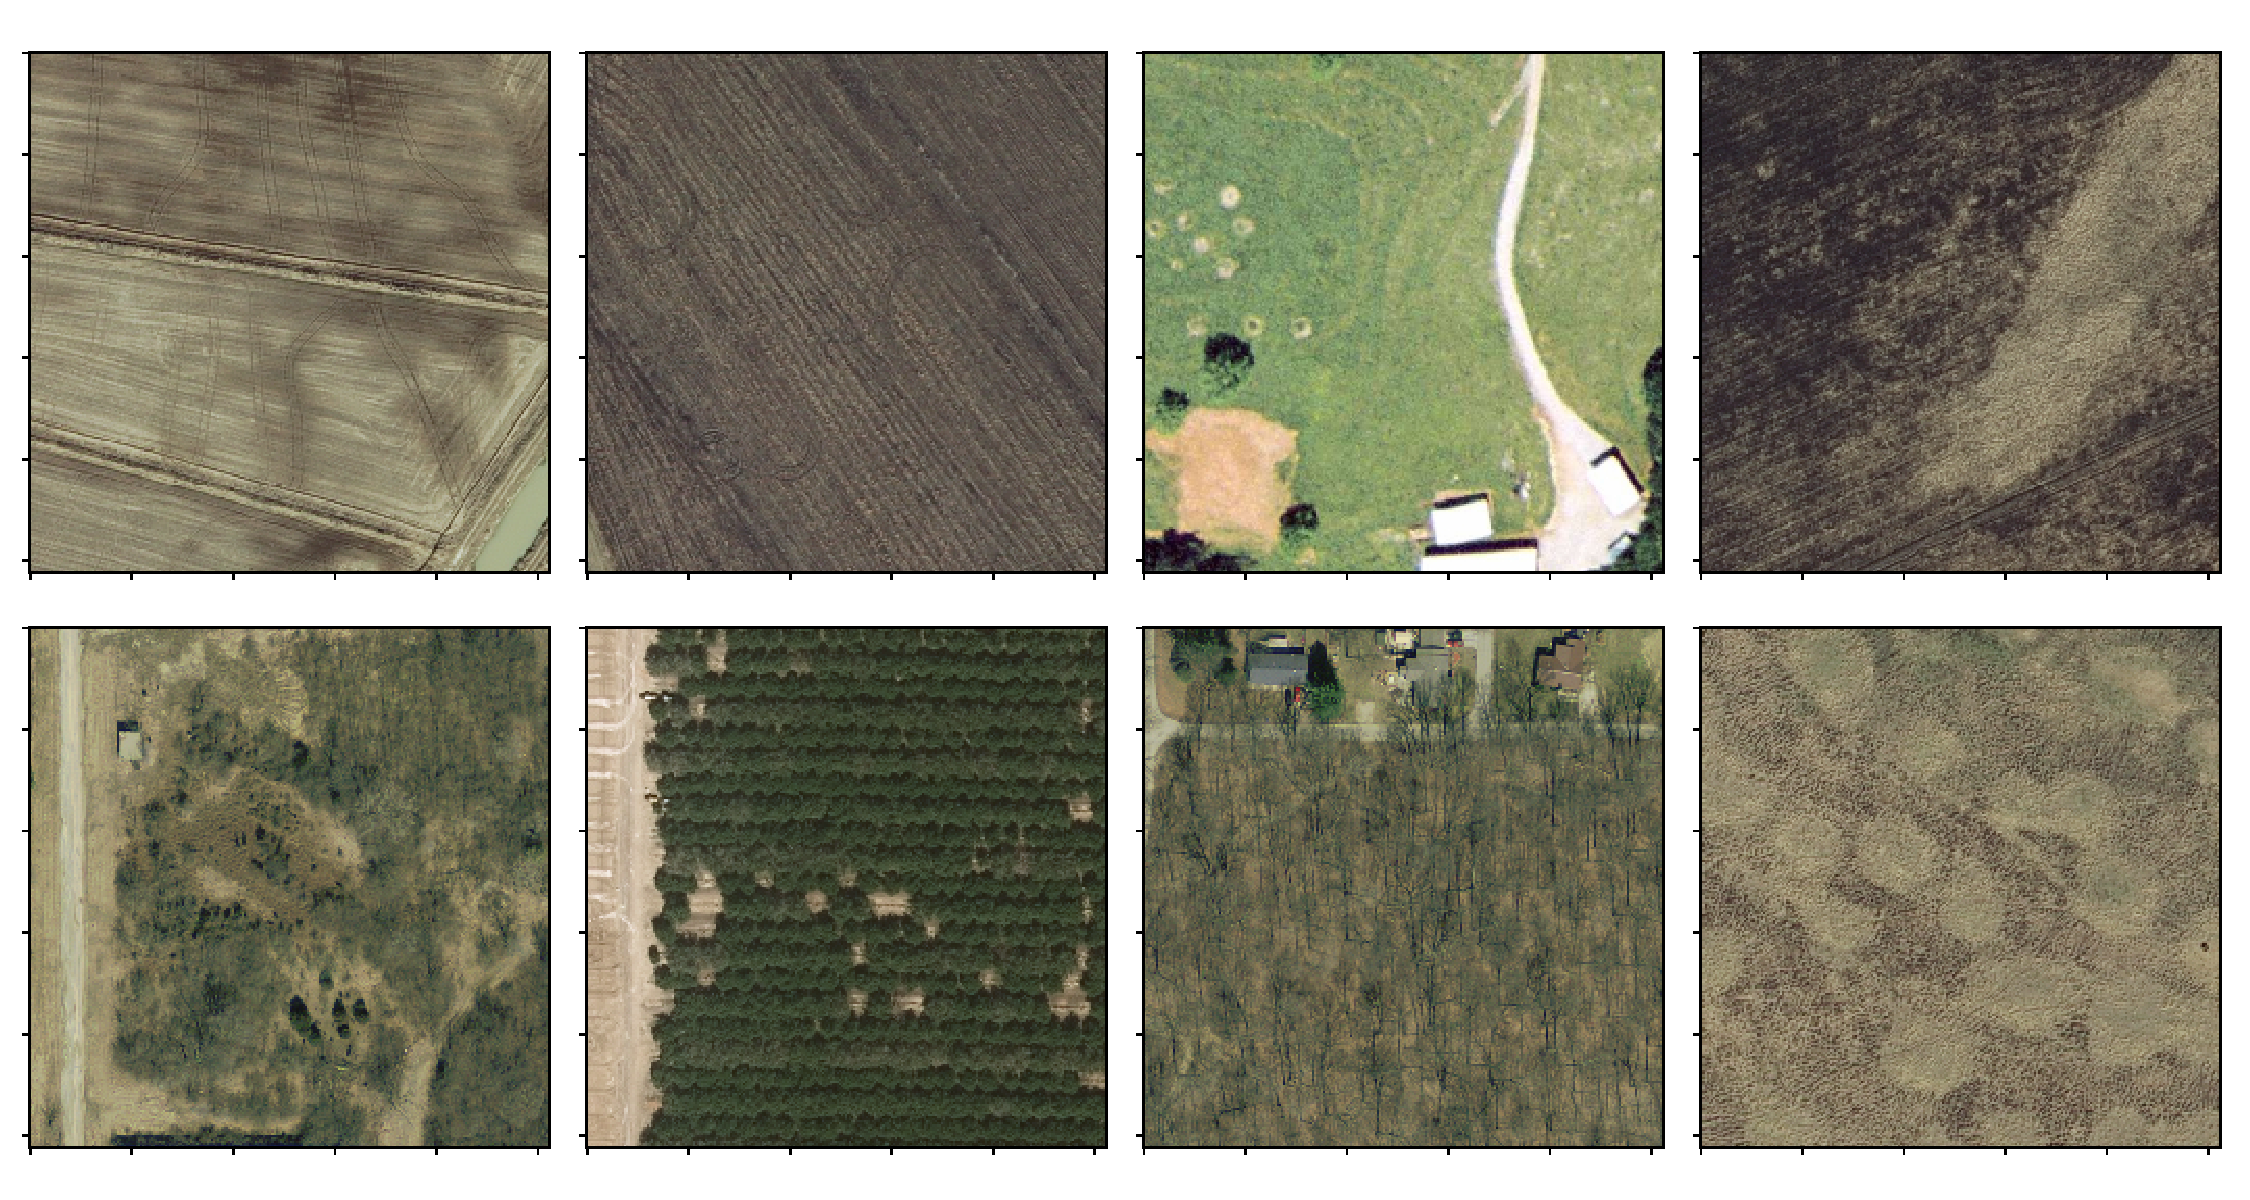
\includegraphics[width=1\textwidth]{Figures/agriculture_sample.pdf}
	\caption{\textbf{Example images of category Agricultue.} All images in this figure show clear signs of human impact. The images have a size of $512\times512$ pixels and a resolution of $0.3$m per pixel.}
	\label{fig:agriculture_sample}
\end{figure}

\begin{figure}[h!]
	\centering
	\captionsetup{width=1\linewidth}
	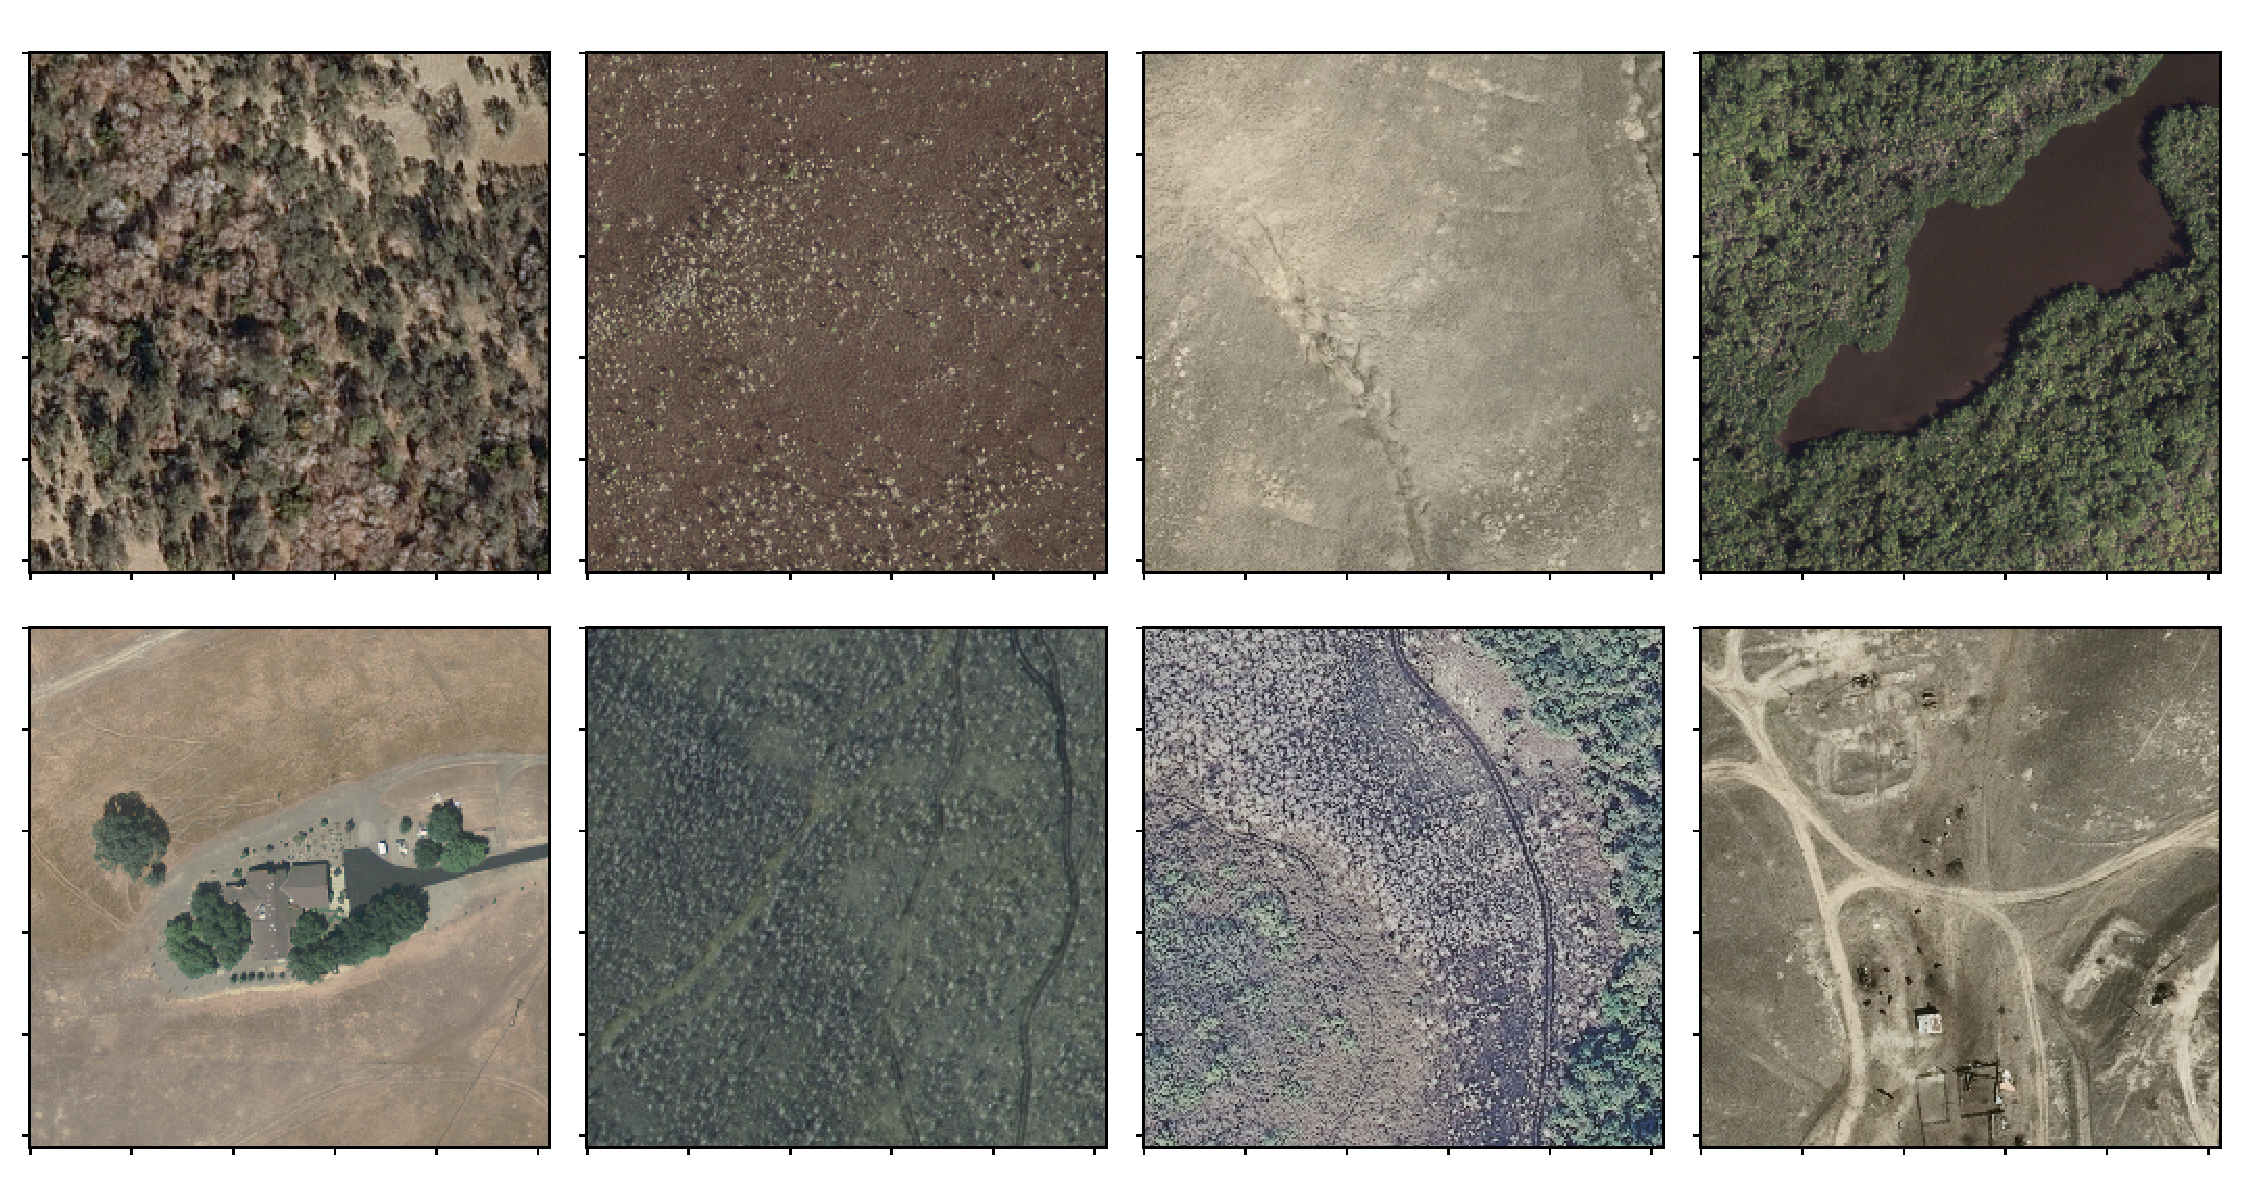
\includegraphics[width=1\textwidth]{Figures/shrubland-grassland_sample.pdf}
	\caption{\textbf{Example images of category Shrubland-grassland.} The images in the first row do not contain any human influence, while the images in the second row show influence by humans. The images in this figure have a size of $512\times512$ pixels and a resolution of $0.3$m per pixel.}
	\label{fig:shrubland-sample}
\end{figure}

\begin{figure}[h!]
	\centering
	\captionsetup{width=1\linewidth}
	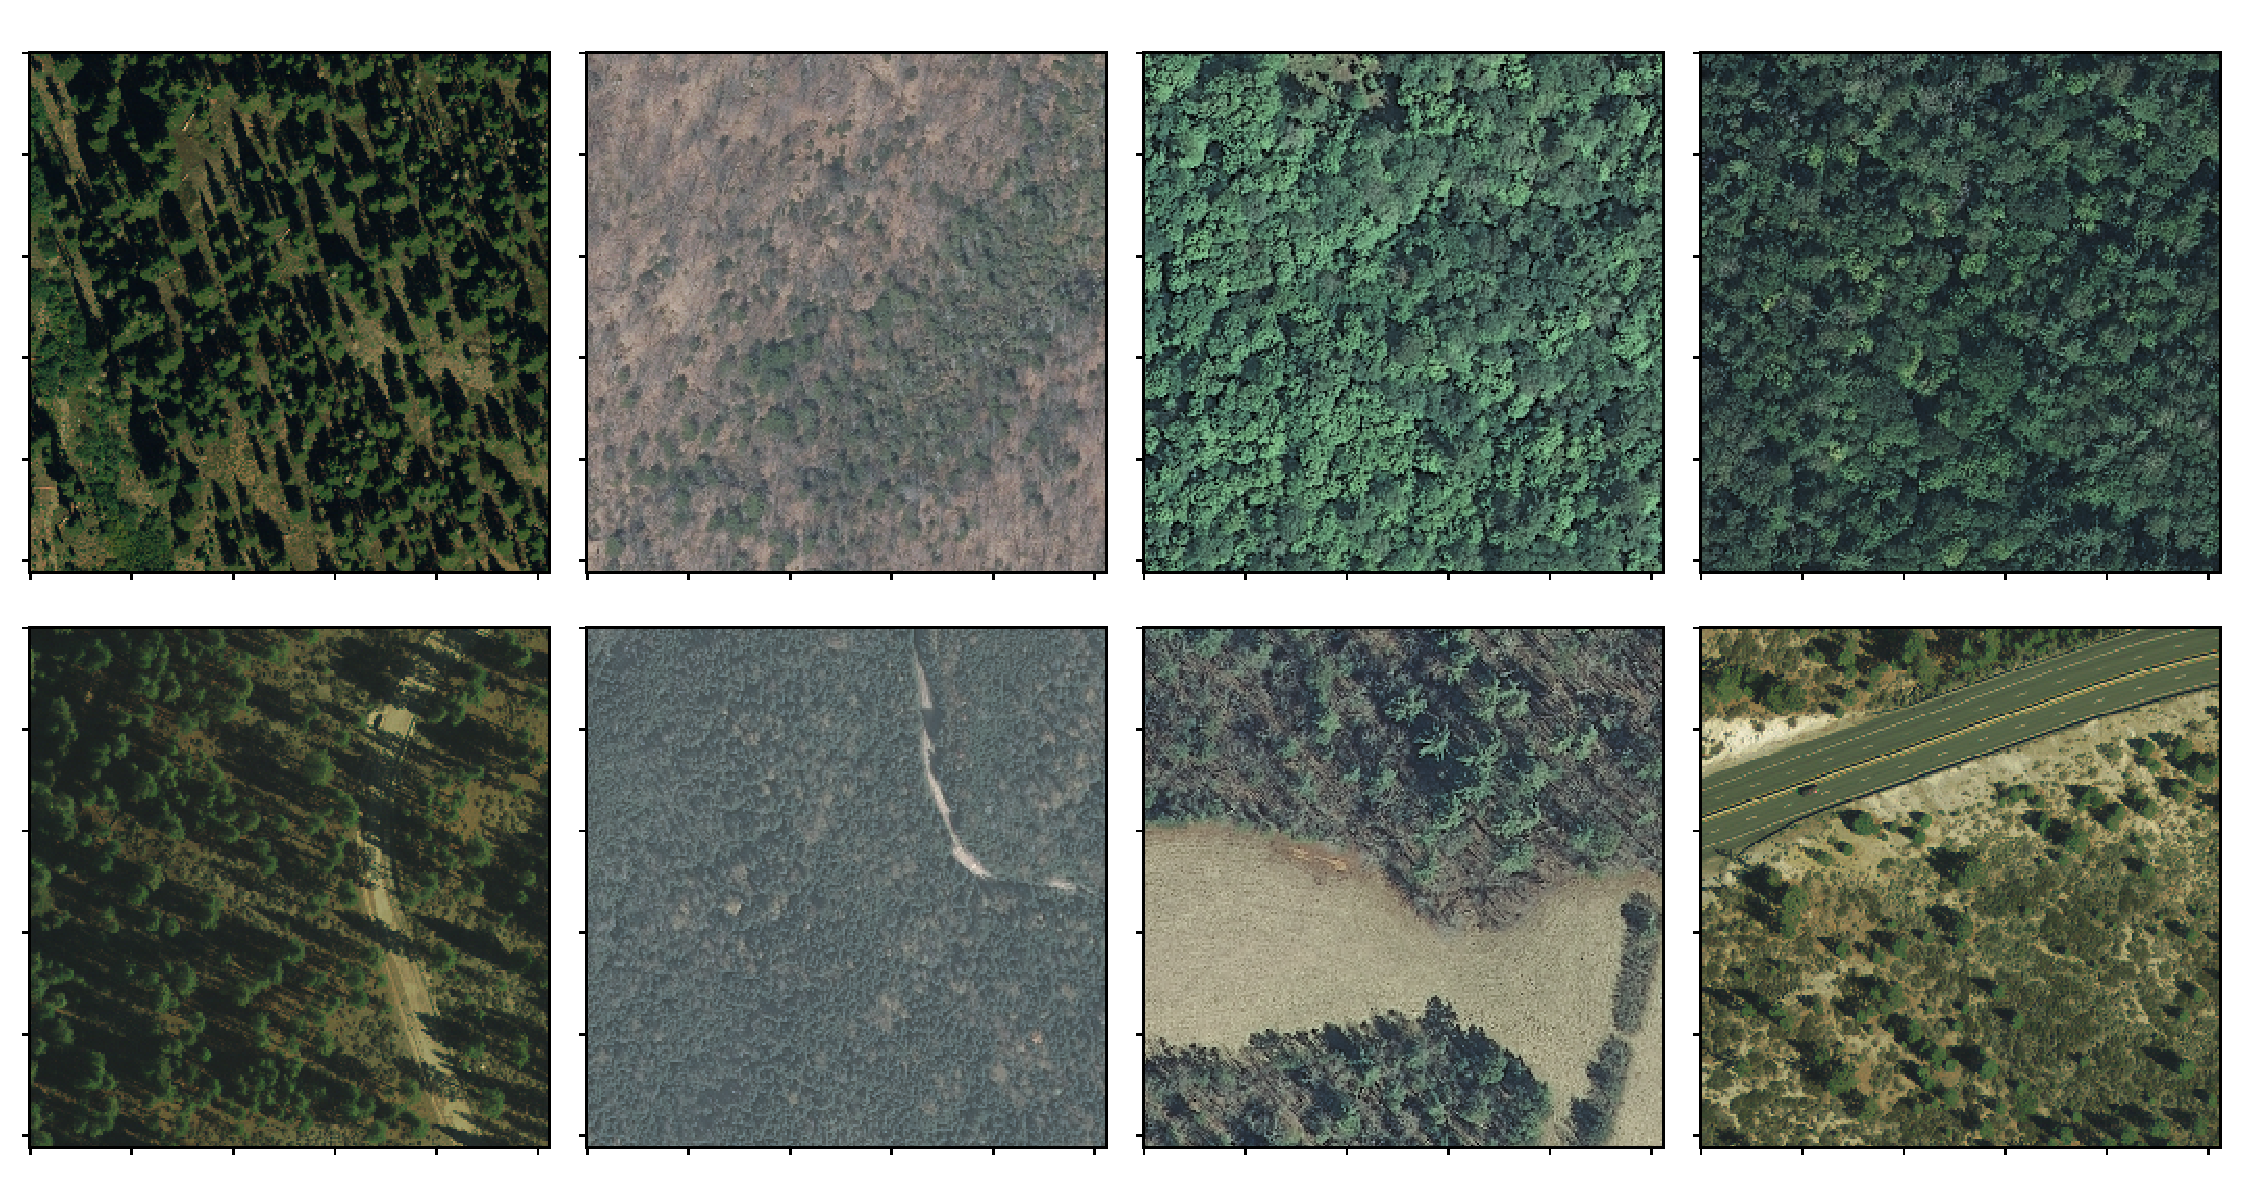
\includegraphics[width=1\textwidth]{Figures/forest-woodland_sample.pdf}
	\caption{\textbf{Example images of category Forest-woodland.} The images in the first row do not contain any human influence, while the images in the second row show influence by humans. The images in this figure have a size of $512\times512$ pixels and a resolution of $0.3$m per pixel.}
	\label{fig:forest-sample}
\end{figure}

\begin{figure}[h!]
	\centering
	\captionsetup{width=1\linewidth}
	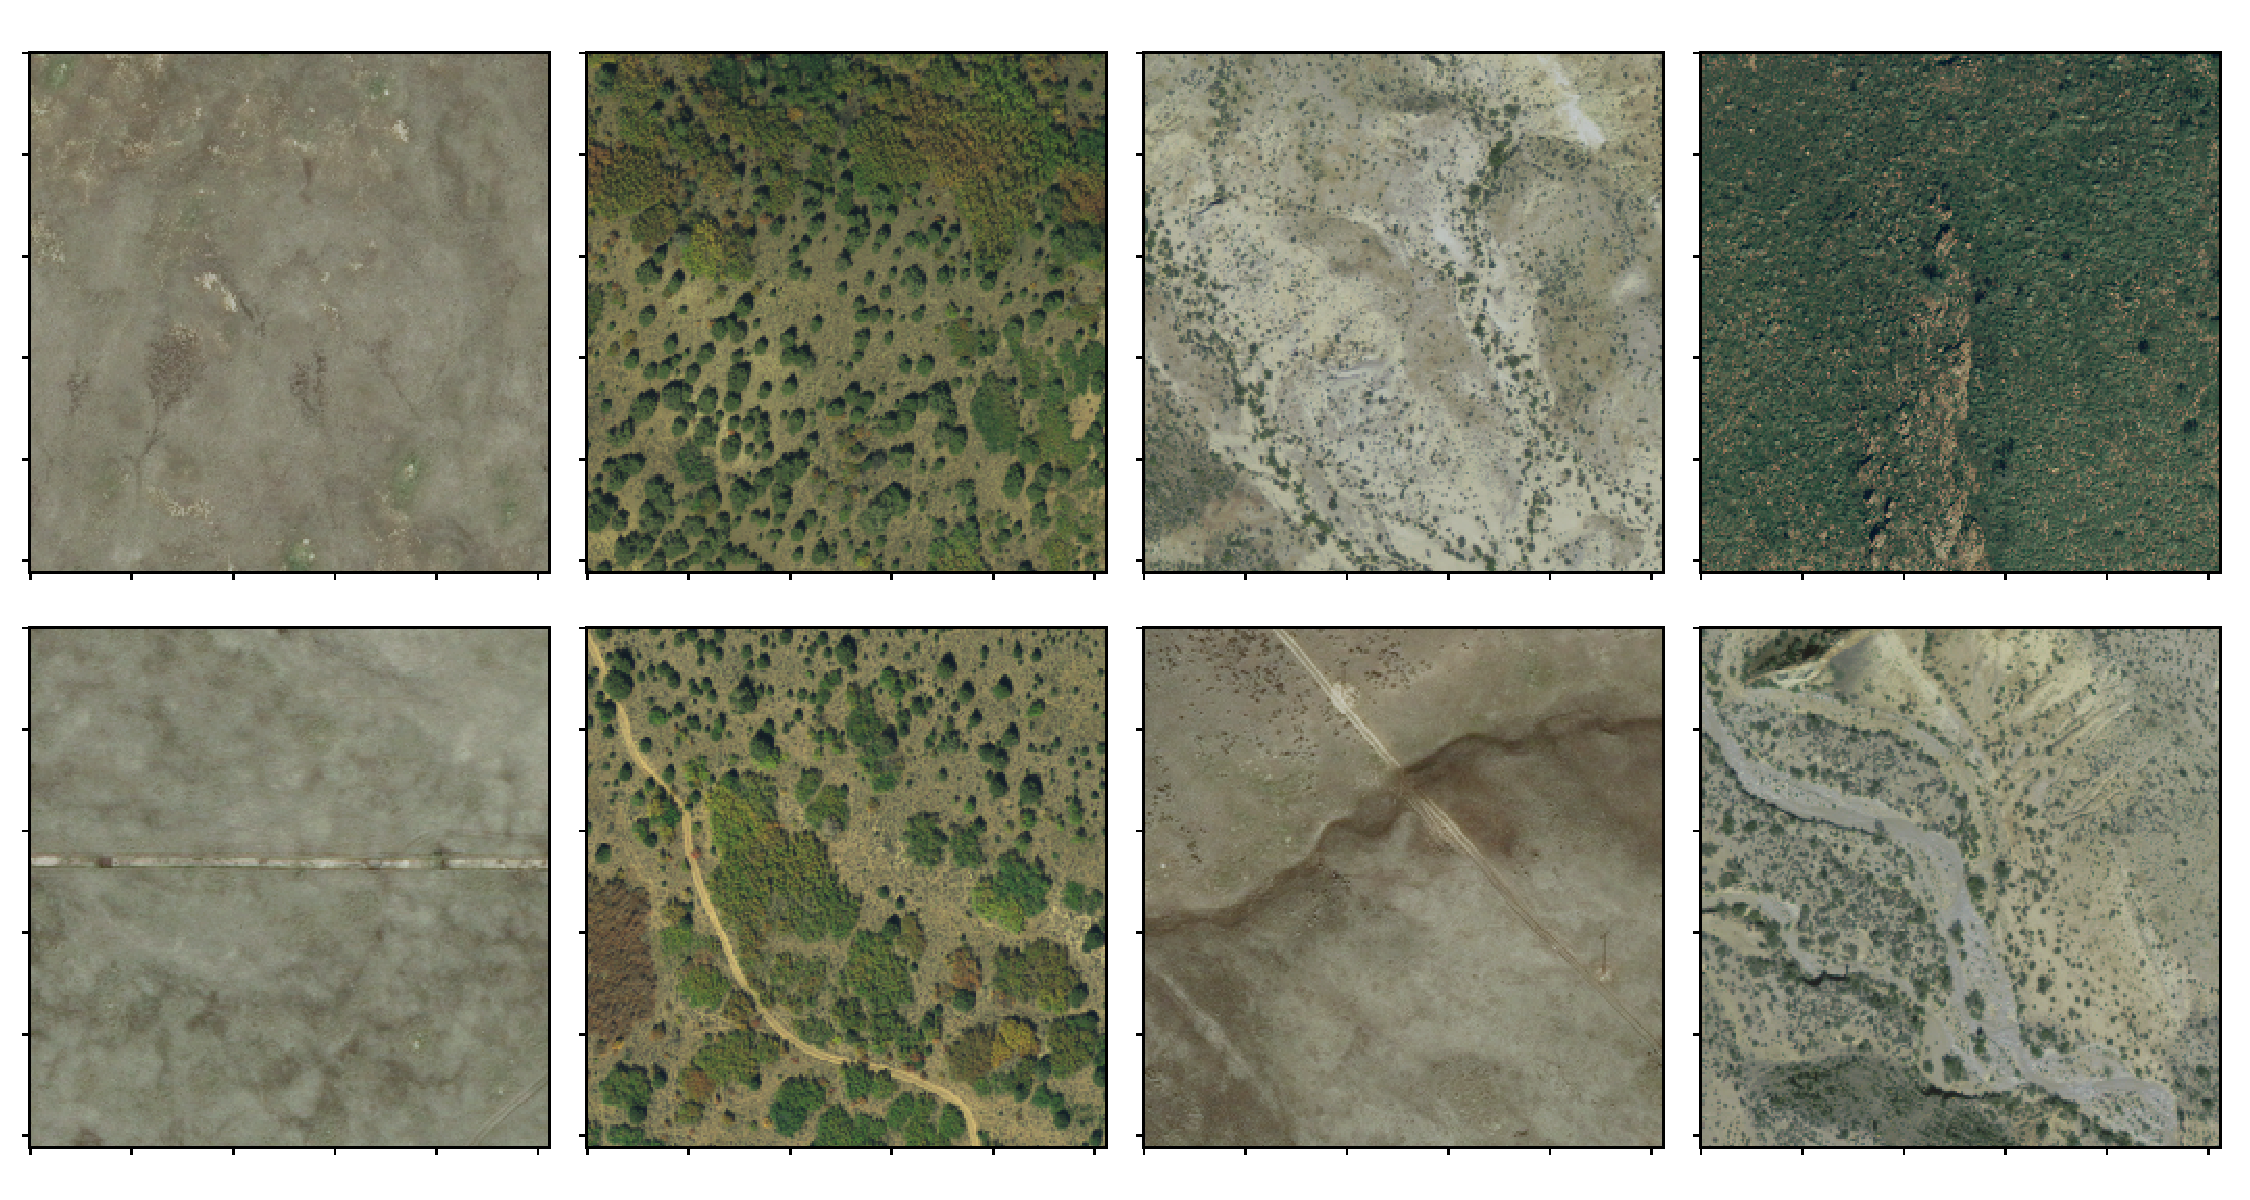
\includegraphics[width=1\textwidth]{Figures/semi-desert_sample.pdf}
	\caption{\textbf{Example images of category Semi-desert.} The images in the first row do not contain any human influence, while the images in the second row show influence by humans. The images in this figure have a size of $512\times512$ pixels and a resolution of $0.3$m per pixel.}
	\label{fig:desert-sample}
\end{figure}

When looking for images we excluded cities and highly developed urban areas, and instead focussed on unpopulated areas. Specifically, we limited our image search to the four Land Use categories Agriculture, Shrubland-Grassland, Semi-Desert, Forest-Woodland that can be found in the USGS Land Cover Viewer. Note that these categories served as a rough geographic reference to pin down geolocations of interest, in order to guarantee a dataset with a good variety of different terrains. We also found that it is harder to find images without human, which is why we selected many images from national parks. However, within a given area/terrain we always tried to have images with and without impact.

Once an area was pointed out as a region of interest, we located it on USGS Earthexplorer and downloaded images from that area. In particular, we constructed two datasets with $0.3m$ and $1m$ resolution, respectively. The former was taken from the category High Resolution Orthoimagery and the latter from the category National Agriculture Imagery Program (NAIP). Note that the images in these categories usually have a height and a width of several thousand pixels, and hence oocupy a few hundreds of Megabytes of disk space. We cropped smaller images out of the raw images, which will be discussed in more detail in the following section. Overall, we downloaded about 100 images for each dataset.


\subsection{Data Processing and Labeling}
Our data processing pipeline consists of the following steps:
\begin{itemize}
	\item Download large raw images
	\item Crop images of size $512\times512$ pixels
	\item Label images with either zero (no human impact), one (minimal human impact), two (obvious human impact)
	\item Degrade images, i.e. reduce number of pixels and thereby resolution per pixel
\end{itemize}

Let us discuss each of these steps in more detail. Every raw image was processed, whereas the processed images of size $512\times512$ were saved in a folder named by its category. Note that every raw image resulted in approximately $100 - 150$ processed images, so that we ended up with more than 10,000 images for each dataset.

Within each category of the processed images we labelled a selected portion of the images, by moving them into the folder with the respective label name. The folder structure we used is the following, where pointy brackets '<parameter>' indicate a parameter and 'etc' stands for the three label folders.

\dirtree{%
	.1 \{raw-images-\}usgs-<pixels>-res<resolution>m.
	.2 semi-desert.
	.3 label-0.
	.3 label-1.
	.3 label-2.
	.2 agriculture.
	.3 label-2.
	.2 shrubland-grassland.
	.3 label-0.
	.3 label-1.
	.3 label-2.
	.2 semi-desert.
	.3 label-0.
	.3 label-1.
	.3 label-2.
}

\begin{figure}[h!]
	\centering
	\captionsetup{width=1\linewidth}
	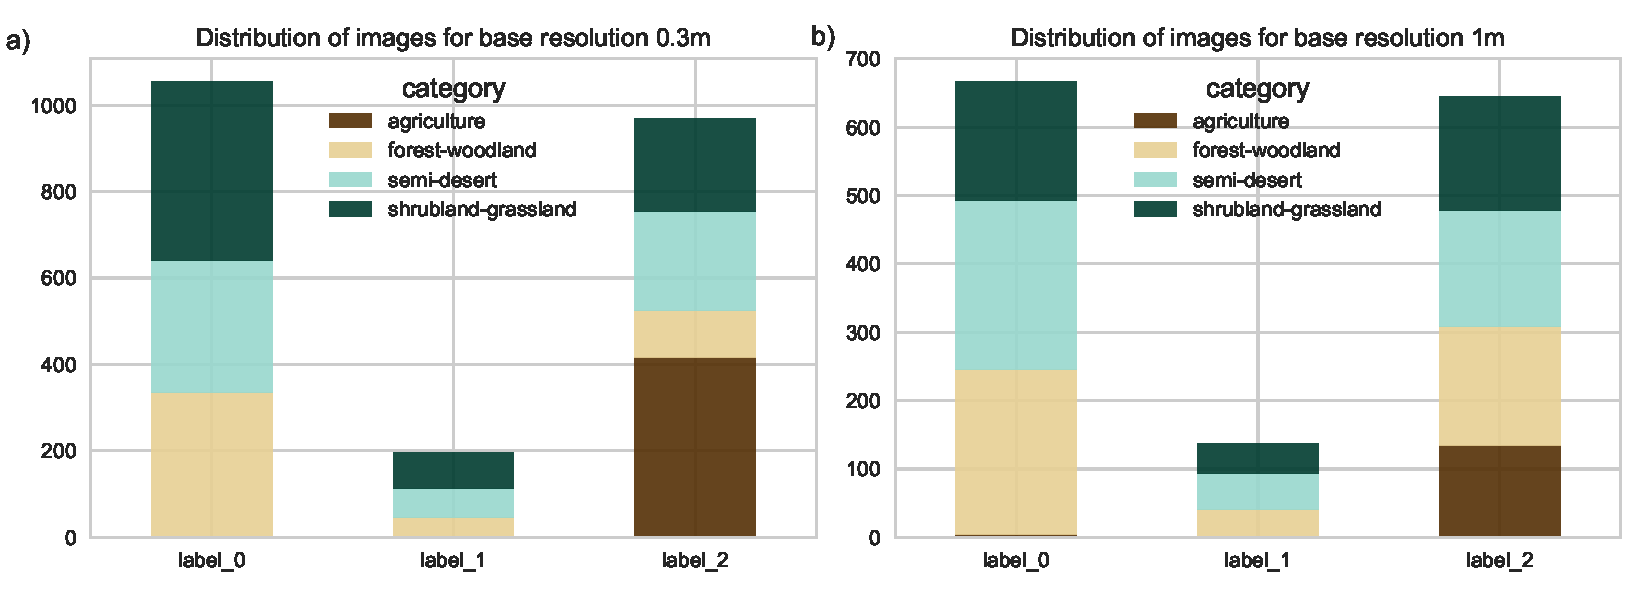
\includegraphics[width=1\textwidth]{Figures/imstats.pdf}
	\caption{\textbf{Number of images per category and label.} (a) Distribution of images for dataset with resolution of 0.3m per pixel. (b) Distribution of images for dataset with resolution of 1m per pixel.}
	\label{fig:imstats}
\end{figure}

When labelling we sticked to the following rules. First, we classified images with no human impact at all into the class with label zero,  while we classified images with very clear human influence into the class with label two. Ambigious images, i.e. images with minimal human trace were classified into label one. Second, we've put major effort into creating datasets that contain images of similar texture spread across all classes. If we for example classified a set of images of a certain forest type into the class with label zero we classified another set of images with a similar forest type, but containing a building or a street, into the class with label two. The same applies for images in class with label one when they contain e.g. a small walking path. We followed the latter rule for all categories except Agriculture. The Agriculture images all show human influence, and were therefore all classified with label two. By sticking to these rules, we are able to guarantee that the algorithm learns features that relate to human impact, and not to image artefacts such as color or texture.

In Figures \ref{fig:agriculture_sample} - \ref{fig:desert-sample} we display sample images for each of the four categories Agriculture, Shrubland-grassland, Forest-woodland and Semi-desert. These images belong to the dataset which has a resolution per pixel of 0.3m. Note that in Figs. \ref{fig:shrubland-sample} - \ref{fig:desert-sample} the first row represents images of label zero and the second row shows images that belong to label two. As mentioned above, the images in Fig.~\ref{fig:agriculture_sample} all contain human influence. 

The distribution of categories and labels is shown in Fig.~\ref{fig:imstats}. Overall, for the 0.3m dataset we classified about 2200 images, and for the 1m dataset we classified about 1450 images. During classification our main goal consisted in creating a balanced dataset between labels zero and two. The minority of images, roughly $10\%$ of all classified images were assigned to label 1. These images were used at random to investigate the behaviour of the Machine Learning classifier, which is discussed in chapter~\ref{Chapter4} \textcolor{red}{VERIFY}.

\begin{figure}[h!]
	\centering
	\captionsetup{width=1\linewidth}
	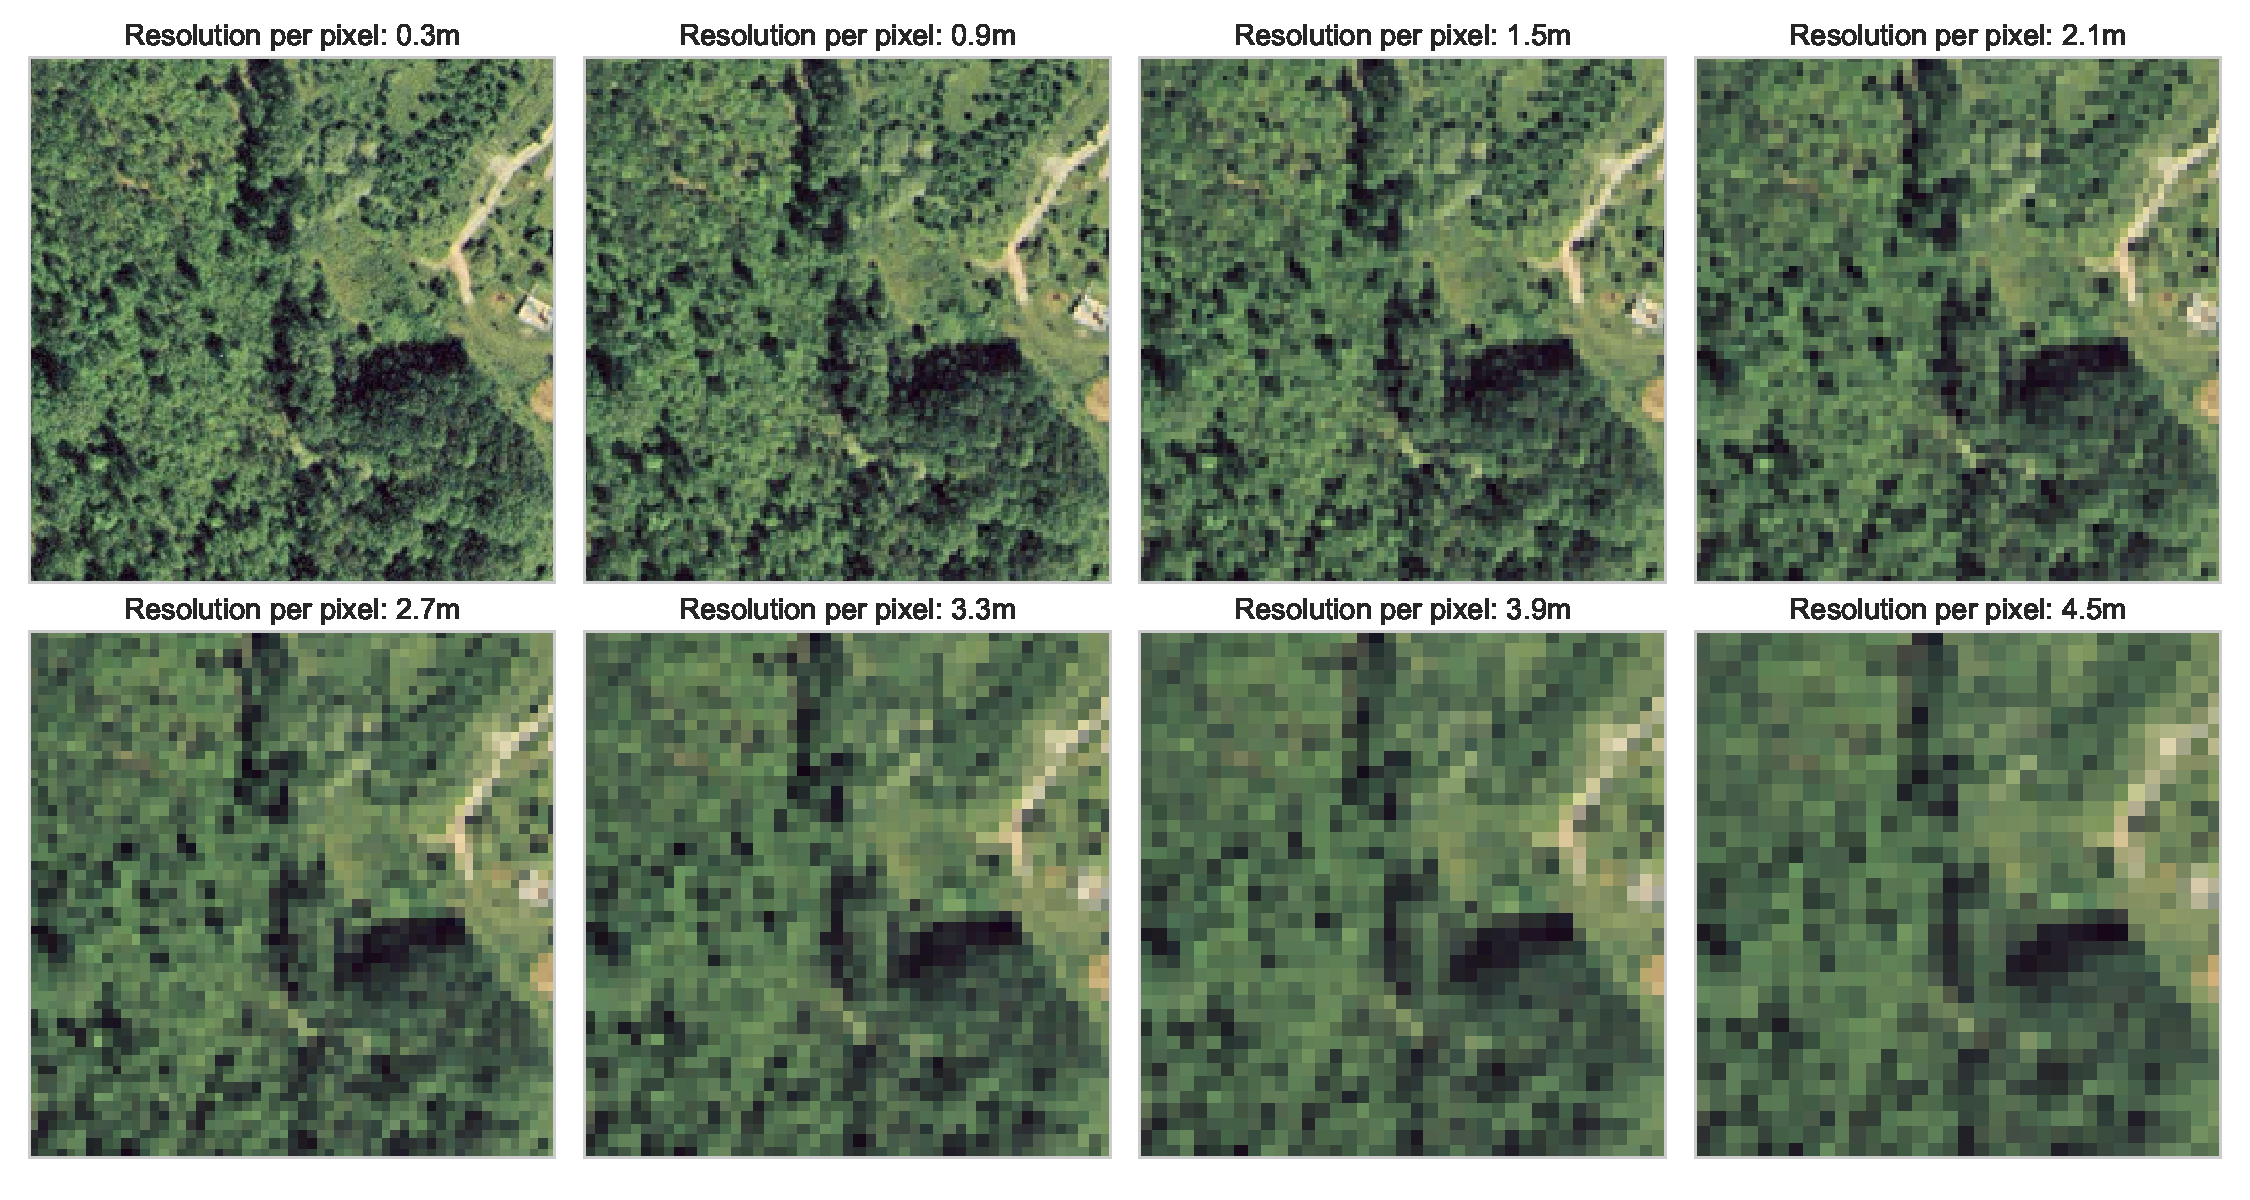
\includegraphics[width=1\textwidth]{Figures/demo_degrade.pdf}
	\caption{\textbf{Example of image downsampling}. The upper left image has the base resolution, 0.3m per pixel, and a size of $512\times512$ pixels whereas the lower right image has the worst resolution, 4.5m per pixel, and a size of $34\times34$ pixels. All intermediate images are downsampled by a factor corresponding to the resolution of the actual image divided by the base resolution. For instance, for the lower right image it is 15.}
	\label{fig:degrade}
\end{figure}

The last step of the data processing pipeline consisted in downsampling the processed and labelled images, to obtain images with a lower resolution per pixel. We used a Lanczos filter \parencite{duchon1979} for the sampling, which is based on a sinusoidal kernel. In Fig.~\ref{fig:degrade}) we show a few selected resolutions for an example image from the agriculture category. Note that here we only schematically depict an example in order to illustrate the process. However, in our Machine Learning pipeline the images are downsampled on the fly and the result of this process is not stored on disk.

For this particular image one can observe how certain image features disappear as the image quality is decreased. Above a resolution of around 3m per pixel one is not able anymore to identify the building close to the right corner of the image. 
The texture of the track that leads up to the building is blurred above a resolution of around 4m per pixel. This shows how different elements in an image are not recognizable anymore once the resolution is worse than their characteristic resolution.



%----------------------------------------------------------------------------------------

%\include{Chapters/Chapter4} 
%\include{Chapters/Chapter5} 

%----------------------------------------------------------------------------------------
%	THESIS CONTENT - APPENDICES
%----------------------------------------------------------------------------------------

\appendix % Cue to tell LaTeX that the following "chapters" are Appendices

% Include the appendices of the thesis as separate files from the Appendices folder
% Uncomment the lines as you write the Appendices

% Appendix A

\chapter{Frequently Asked Questions} % Main appendix title

\label{AppendixA} % For referencing this appendix elsewhere, use \ref{AppendixA}

\section{How do I change the colors of links?}

The color of links can be changed to your liking using:

{\small\verb!\hypersetup{urlcolor=red}!}, or

{\small\verb!\hypersetup{citecolor=green}!}, or

{\small\verb!\hypersetup{allcolor=blue}!}.

\noindent If you want to completely hide the links, you can use:

{\small\verb!\hypersetup{allcolors=.}!}, or even better: 

{\small\verb!\hypersetup{hidelinks}!}.

\noindent If you want to have obvious links in the PDF but not the printed text, use:

{\small\verb!\hypersetup{colorlinks=false}!}.

%\include{Appendices/AppendixB}
%\include{Appendices/AppendixC}

%----------------------------------------------------------------------------------------
%	BIBLIOGRAPHY
%----------------------------------------------------------------------------------------

\printbibliography[heading=bibintoc]


%----------------------------------------------------------------------------------------

\end{document}  
